\section{Cân bằng trong dung dịch nước}
\begin{Muctieu}
	\begin{itemize}
		\item  Nêu được khái niệm sự điện li, chất điện li, chất không điện li.
		\item  Trình bày được thuyết Brønsted - Lowry (Bron-stêt - Lau-ri) về acid - base.
		\item  Nêu được khái niệm và ý nghĩa của pH trong thực tiễn (liên hệ giá trị pH ở các bộ phận trong cơ thể với sức khoẻ con người, pH của đất, nước tới sự phát triển của động thực vật, ...).
		\item  Viết được biểu thức tính pH và biết cách sử dụng các chất chỉ thị để xác định pH (môi trường acid, base, trung tính) bẳng các chất chỉ thị phổ biến như giấy chi thị màu, quỳ tím, phenolphthalein, ...
		\item  Nêu được nguyên tắc xác định nồng độ acid, base mạnh bằng phương pháp chuẩn độ.
		\item  Thực hiện được thí nghiệm chuẩn độ acid - base: Chuẩn độ dung dịch base mạnh (sodium hydroxide) bằng dung dich acid mạnh (hydrochloric acid).
		\item  Trình bày được ý nghĩa thực tiễn cân bằng trong dung dịch nước của ion $\mathrm{Al}^{3+}, \mathrm{Fe}^{3+}$ $\mathrm{Và}_{\mathrm{Cl}} \mathrm{CO}_3^{2-}$.
	\end{itemize}
\end{Muctieu}
\subsection{Nội dung bài học}
\begin{kd}
	\immini{Có một anh kĩ sư nông nghiệp trồng cà chua. Anh ấy nhận thấy cây cà chua của mình không phát triển tốt như mong đợi. Sau khi tìm hiểu, anh ấy biết rằng cà chua thích hợp với đất có độ pH từ $6{,}0$ đến $6{,}8$. Anh ấy đo pH của đất trong vườn và thấy nó là $5{,}5$.
		Câu hỏi đặt ra là:
		\begin{itemize}
			\item Tại sao độ pH của đất lại quan trọng đối với sự phát triển của cây trồng?
			\item Điều gì khiến độ pH của đất thay đổi?
			\item Làm thế nào để anh kĩ sư nông nghiệp có thể điều chỉnh pH của đất?
		\end{itemize}
		}{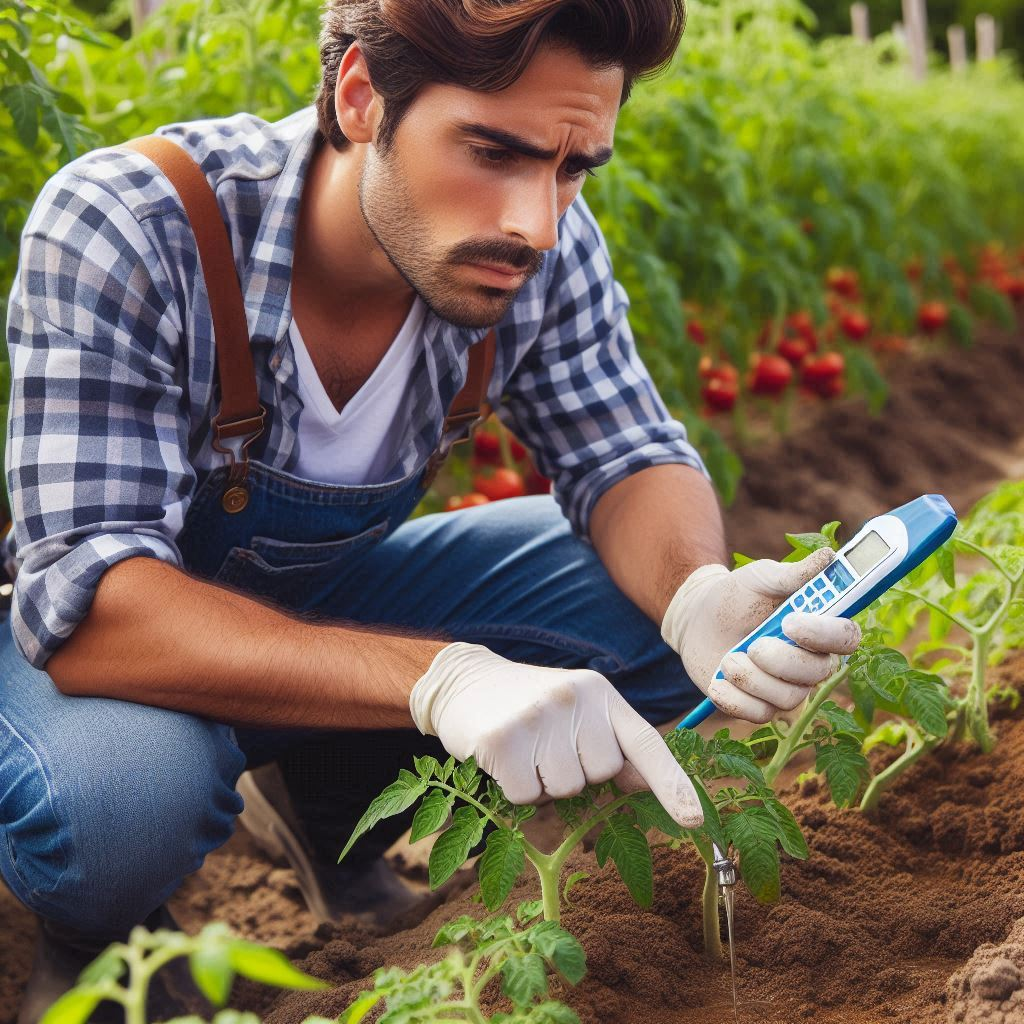
\includegraphics[width=5cm]{Images/anhhoa11/dopH.jpg}}
		Để trả lời những câu hỏi này, chúng ta cần hiểu về cân bằng axit-bazơ trong dung dịch, đặc biệt là trong môi trường đất. Đất là một hệ thống phức tạp, trong đó có nhiều phản ứng hóa học xảy ra đồng thời, bao gồm cả các phản ứng cân bằng.
\end{kd}
\subsubsection{Sự điện li}
\Noibat[\maunhan]{Hiện tượng điện li}
\Noibat[][][\faApple]{Tìm hiểu về sự điện li}
\begin{figure}[!htp]
	\begin{hopdongian}[\mauphu]
		{\indam[\mauphu]{\faAsterisk\;Thí nghiệm về sự điện li}
			\begin{itemize}
				\item \textbf{Chuẩn bị hóa chất:} Kim loại: $Al$, $Cu$; muối: $NaCl$, $CaCl_2$, $CuSO_4$; hạt nhựa PVC, đường, rượu etylic, silic dioxit.
				\item \textbf{Cách tiến hành:}
				\begin{itemize}
					\item Thí nghiệm 1: Đặt điện cực tiếp xúc trực tiếp với các chất trước khi cho nước cất vào.
					\item Thí nghiệm 2: Đặt điện cực tiếp xúc với nước sau khi rót nước vào và khuấy đều.
				\end{itemize}
				Quan sát hiện tượng.
			\end{itemize}
		}
		\begin{center}
			\begin{subfigure}[b]{0.23\textwidth}
				\centering
				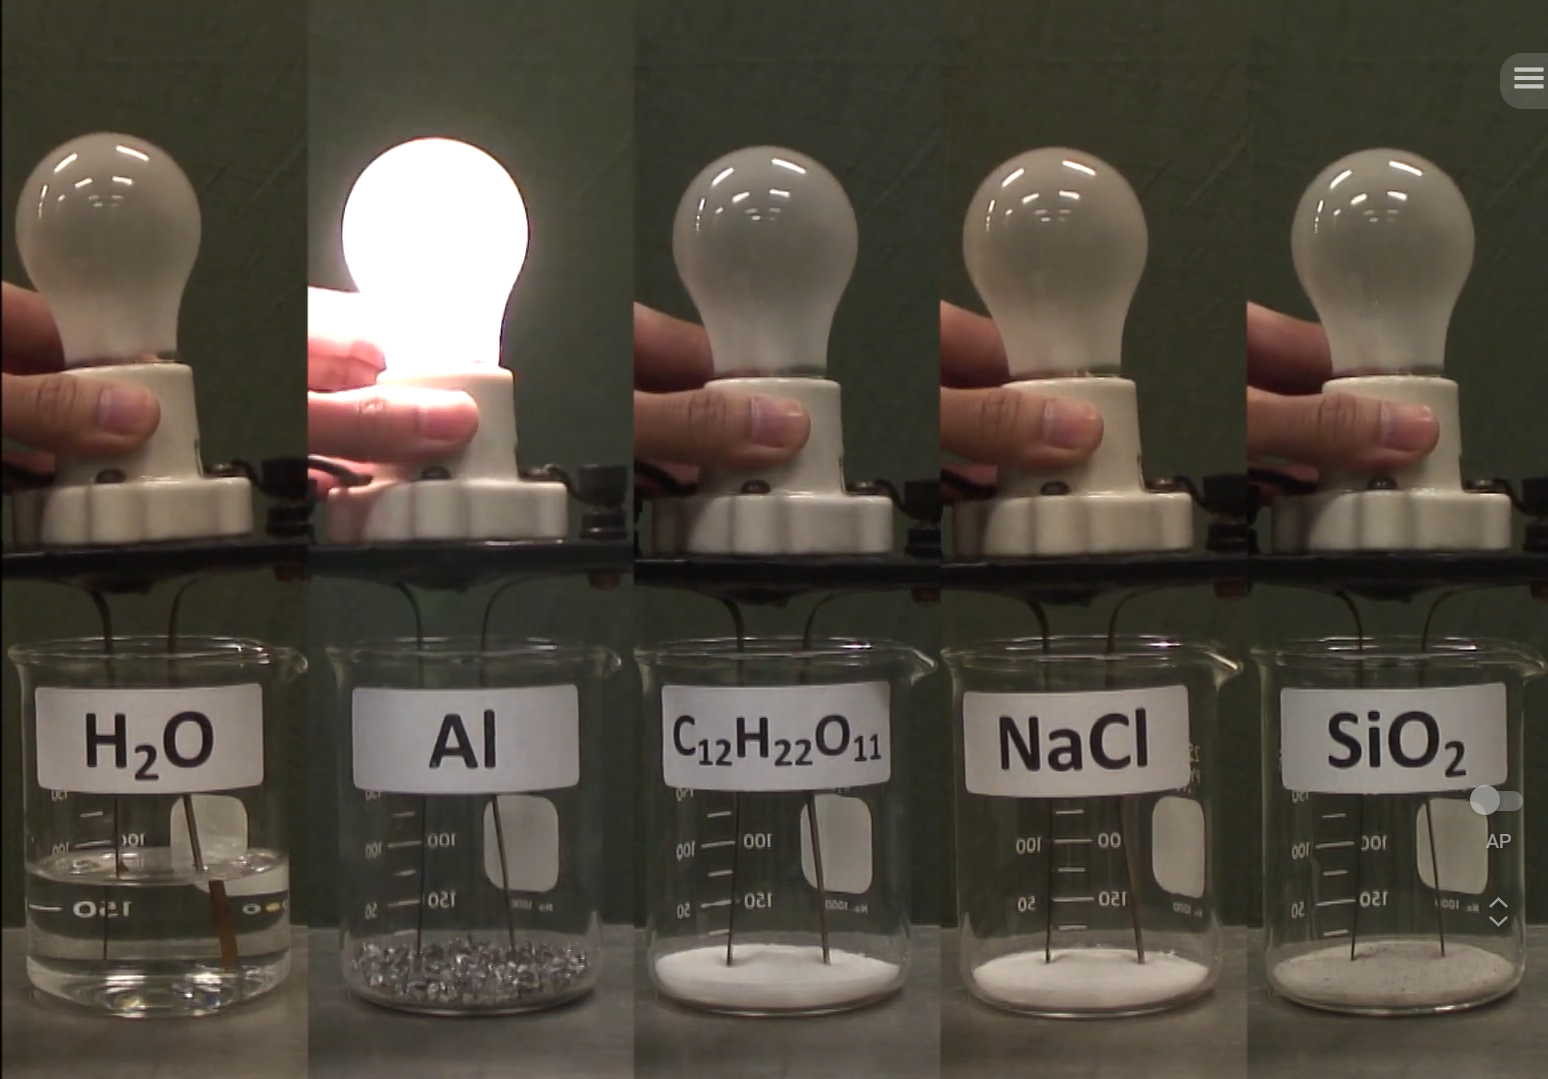
\includegraphics[height=0.7\textwidth]{Images/anhhoa11/dodandien_1.png}
				\caption{Trước khi rót nước vào}
				\label{subfig:TNsudienli1}
			\end{subfigure}
			\begin{subfigure}[b]{0.23\textwidth}
				\centering
				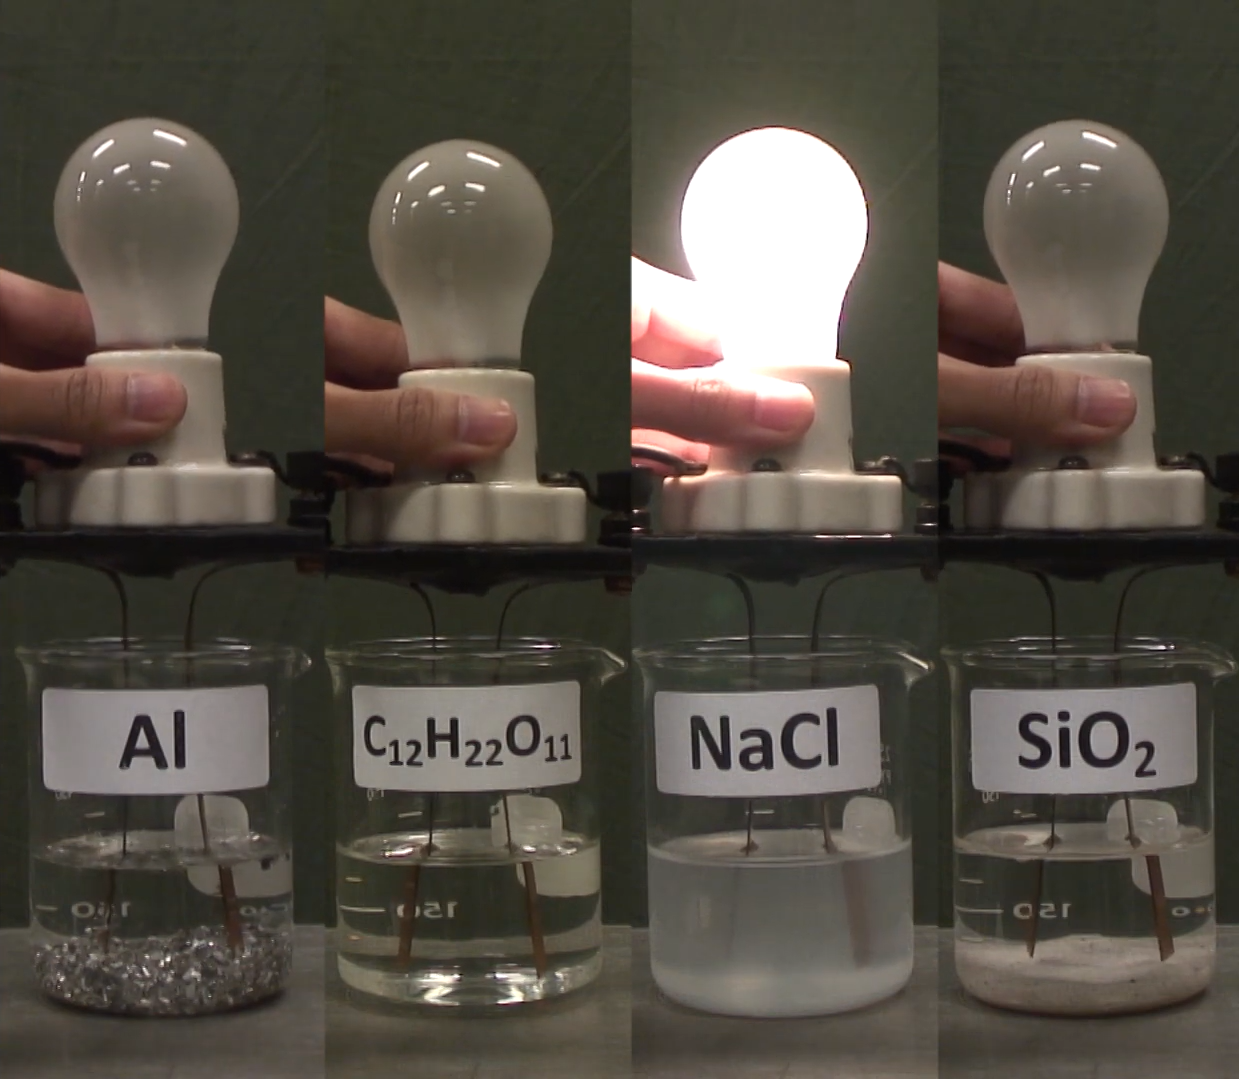
\includegraphics[height=0.7\textwidth]{Images/anhhoa11/dodandien_2.png}
				\caption{Đã rót nước và khuấy}
				\label{subfig:TNsudienli2}
			\end{subfigure}
			\hspace*{0.5cm}
			\begin{subfigure}[b]{0.23\textwidth}
				\centering
				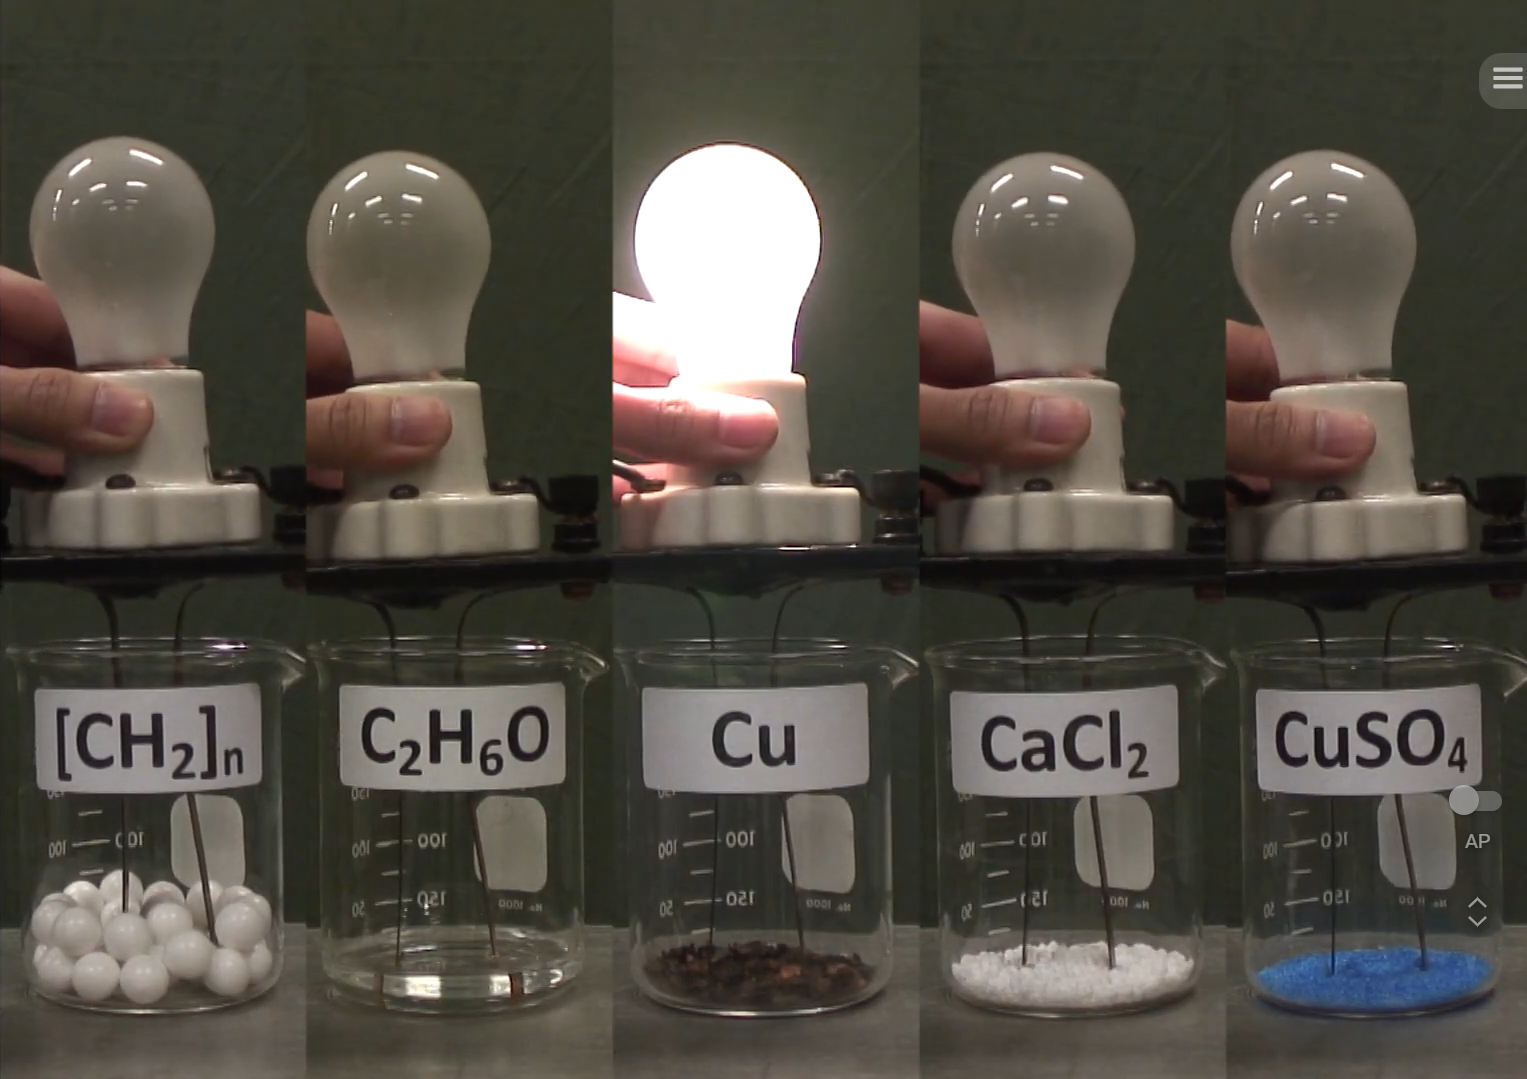
\includegraphics[height=0.7\textwidth]{Images/anhhoa11/dodandien_3.png}
				\caption{Trước khi rót nước vào}
				\label{subfig:TNsudienli3}
			\end{subfigure}
			\hspace*{0.25cm}
			\begin{subfigure}[b]{0.23\textwidth}
				\centering
				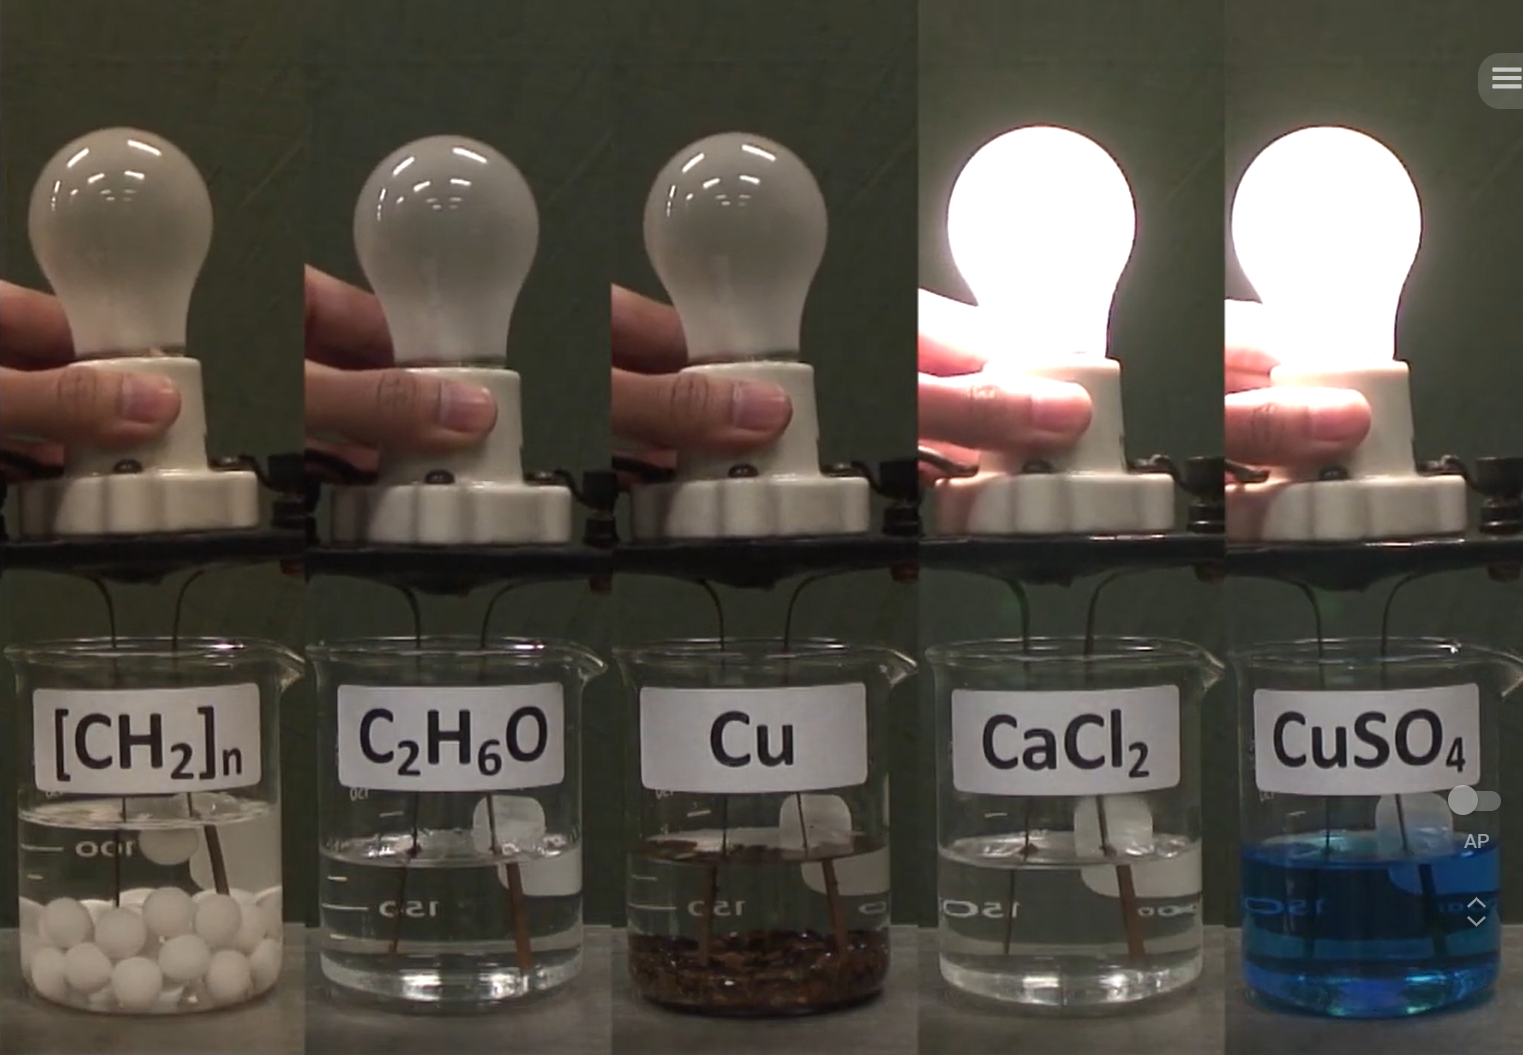
\includegraphics[height=0.7\textwidth]{Images/anhhoa11/dodandien_4.png}
				\caption{Đã cho nước và khuấy}
				\label{subfig:TNsudienli4}
			\end{subfigure}
			\caption{Thí nghiệm về sự điện li}
			\label{fig:TNsudienli}
		\end{center}
	\end{hopdongian}
\end{figure}
\begin{hoivadap}
	\begin{cauhoi}
		Quan sát ở hình \ref{fig:TNsudienli} hãy trả lời các câu hỏi sau:
	    \begin{enumerate}[(1)]
	    	\item Trước khỉ rót nước vào (thí nghiệm 1), bóng đèn có sáng khi nhúng cặp điện cực vào các chất nào? Tại sao?
	    	Đối với các chất không làm sáng bóng đèn trong thí nghiệm 1, bạn có nhận xét gì về trạng thái của chúng (rắn, lỏng, khí)?
	    	\item Sau khi hòa tan các chất vào nước và khuấy đều (thí nghiệm 2), bóng đèn có sáng khi nhúng cặp điện cực vào dung dịch nào? 
	    	\item So sánh kết quả của thí nghiệm 1 và thí nghiệm 2. Bạn nhận thấy điều gì khác biệt?
	    	\item Đối với các chất làm sáng bóng đèn trong thí nghiệm 2 nhưng không làm sáng trong thí nghiệm 1, điều gì đã xảy ra khi chúng được hòa tan vào nước?Theo bạn, tại sao một số chất chỉ dẫn điện khi được hòa tan vào nước?
	    	\item Nếu một chất khi hòa tan vào nước làm cho dung dịch dẫn điện, bạn nghĩ trong dung dịch đó có gì?
	    \end{enumerate}
	\end{cauhoi}
	\loigiai{%
		\begin{enumerate}[(1)]
			\item Trong thí nghiệm 1 trước khỉ rót nước vào, bóng đèn sáng khi nhúng cặp điện cực vào kim loại $Al$, $Cu$. Đây là do kim loại  có cấu trúc tinh thể với các electron tự do có thể di chuyển, cho phép dòng điện đi qua.
			Các chất không làm sáng bóng đèn như (nước cất,nhựa PVC, rượu, canxi clorua rắn, đồng sunfat khan,...) đều ở trạng thái rắn hoặc lỏng, nhưng không có cấu trúc cho phép các hạt mang điện di chuyển tự do.
			\item Trong thí nghiệm 2, sau khi hòa tan các chất vào nước và khuấy đều, bóng đèn sáng khi nhúng cặp điện cực vào dung dịch Natri clorua,canxi clorua và dung dịch đồng sunfat.
			\item So sánh kết quả của hai thí nghiệm, ta nhận thấy:
			\begin{itemize}
				\item Thí nghiệm 1: Chỉ có kim loại đồng, nhôm dẫn điện.
				\item Thí nghiệm 2: dung dịch natri clorua,canxi clorua và đồng sunfat  dẫn điện.
			\end{itemize}
			Điều này cho thấy một số chất không dẫn điện ở trạng thái rắn, nhưng lại dẫn điện khi hòa tan trong nước.
			\item Khi Natriclorua, canxi clorua và đồng sunfat được hòa tan vào nước, chúng phân li thành các ion. Các ion này có khả năng di chuyển tự do trong dung dịch, cho phép dòng điện đi qua. Một số chất chỉ dẫn điện khi hòa tan trong nước vì nước có khả năng phân li các chất thành các ion mang điện.
			\item Khi một chất hòa tan vào nước làm cho dung dịch dẫn điện, trong dung dịch đó có các ion. Các ion này là các hạt mang điện có khả năng di chuyển tự do trong dung dịch, cho phép dòng điện đi qua. Ví dụ, trong dung dịch canxi clorua, ta có các ion $Ca^{2+}$ và $Cl^-$, còn trong dung dịch đồng sunfat, ta có các ion $Cu^{2+}$ và $SO4^{2-}$.
		\end{enumerate}}
\end{hoivadap}
\begin{tomtat}
	Quá trình phân li các chất trong nước tạo thành ion được gọi là \indam{sự điện li}.
\end{tomtat}
\Noibat[\maunhan]{Chất điện li}
\Noibat[\mauphu][][\faArrowCircleORight]{Chất điện li và chất không điện li}
\\
Thí nghiệm trên cho thấy: các chất như natri clorua, canxi clorua,... tan trong nước phân li ra các ion nên chúng là chất điện li. Saccarose, ethanol,... không phân li ra các ion nên chúng là chất không điện li.
\\
Như vậy trong dung dịch $NaCl$ có chứa các ion $Na^+$ và $Cl^-$ mang điện còn ở dung dịch đường chức các phân tử đường không mang điện
\begin{equation}\label{eq:dienliNaCl}
	\mathrm{NaCl}(s) \rightarrow \mathrm{Na}^{+}(a q)+\mathrm{Cl}^{-}(a q)
\end{equation}
\begin{equation}
	\mathrm{C}_{12} \mathrm{H}_{22} \mathrm{O}_{11}(s) \rightarrow \mathrm{C}_{12} \mathrm{H}_{22} \mathrm{O}_{11}(a q)
\end{equation}
Phương trình (\ref{eq:dienliNaCl}) được gọi là \indam{phương trình điện li}
\vspace{0.25cm}
\begin{tomtat}
	 \begin{itemize}
	 	\item Những chất khi tan trong nước phân li ra các ion được gọi là \indam{chất điện li}
	 	\item Những chất khi tan trong nước không phân li thành các ion được gọi là \indam{Chất không diện li} .
	 \end{itemize}
\end{tomtat}
\Noibat[\mauphu][][\faArrowCircleORight]{Chất điện li mạnh và chất điện li yếu}
\begin{figure}[!htp]
	\begin{hopdongian}[\mauphu]
		{\indam[\mauphu]{\faAsterisk\;Thí nghiệm so sánh khả năng phân li trong nước của $HCl$ và $CH_3COOH$}\\
		- Chuẩn bị 2 dung dịch $\mathrm{HCl}$ $0{,}1\mathrm{M}$ và dung dịch $\mathrm{CH}_3\mathrm{COOH}$ $0{,}1\mathrm{M}$, cắm điện cực vào 2 dung dịch , quan sát hiện tượng xảy ra?
		}
		\begin{center}
			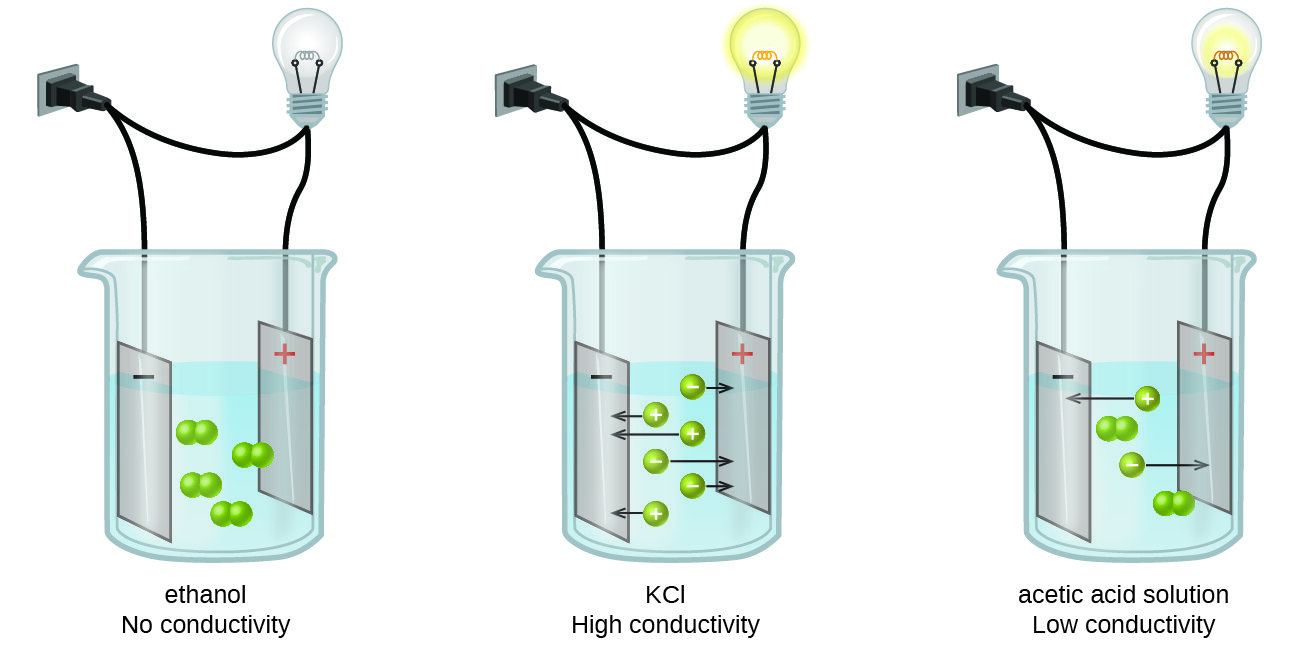
\includegraphics[width=5.5cm,trim={6cm 0cm 0cm 0cm},clip]{Images/anhhoa11/dodandien.jpg}
			\caption{Thí nghiệm so sánh khả năng phân li của $HCl$ và $CH_3COOH$}
			\label{fig:ssdodienli}
		\end{center}
	\end{hopdongian}
\end{figure}
\begin{hoivadap}
	\begin{cauhoi}
		Quan sát và nêu hiện tượng của thí nghiệm?Giải thích
	\end{cauhoi}
		\loigiai{%
		\\
		\textbf{Hiện tượng}:
		Cả hai dung dịch đều dẫn điện, nhưng dung dịch $\mathrm{HCl} 0,1 \mathrm{M}$ dẫn điện tốt hơn dung dịch $\mathrm{CH}_3\mathrm{COOH} 0,1 \mathrm{M}$.\\
		\textbf{Giải thích}:
	\begin{itemize}
		\item Cả $\mathrm{HCl}$ và $\mathrm{CH}_3\mathrm{COOH}$ đều là axit, khi hòa tan trong nước sẽ điện ly tạo ra các ion:
		\begin{align*}
		\mathrm{HCl} \rightarrow \mathrm{H}^+ + \mathrm{Cl}^-\\
		\mathrm{CH}_3\mathrm{COOH} \rightleftharpoons \mathrm{CH}_3\mathrm{COO}^- + \mathrm{H}^+
		\end{align*}
		\item Độ dẫn điện của dung dịch phụ thuộc vào số lượng ion trong dung dịch. Dung dịch có nhiều ion hơn sẽ dẫn điện tốt hơn.Khi nhúng điện cực vào dung dịch $HCl$ đèn sáng mạnh hơn so với dung dịch $CH_3COOH$, điều đó chứng tỏ $HCl$ khi hòa tan vào nước phân li ra nhiều ion hơn so với $CH_3COOH$
		\item \textbf{Kết luận:} Dung dịch $\mathrm{HCl} 0{,}1 \mathrm{M}$ dẫn điện tốt hơn dung dịch $\mathrm{CH}_3\mathrm{COOH} 0{,}1 \mathrm{M}$ vì $\mathrm{HCl}$ là axit mạnh, điện ly hoàn toàn, tạo ra nhiều ion hơn trong dung dịch so với $\mathrm{CH}_3\mathrm{COOH}$ - một axit yếu chỉ điện ly một phần.
	\end{itemize}
	}
\end{hoivadap}
\vspace*{0.25cm}
\begin{tomtat}
	Dựa vào mức độ phân li thành các ion, chất điện li được chia thành hai loại:
	\begin{enumerate}
	\item \indam{Chất điện li mạnh} là chất khi tan trong nước, hầu hết các phân tử chất tan đều phân li ra ion. Các chất điện li mạnh thường gặp là:
\begin{itemize}
		\item \textbf{Các acid mạnh:} $\mathrm{HCl}, \mathrm{HNO}_3, \mathrm{H}_2 \mathrm{SO}_4, \ldots$
		\item \textbf{Các base mạnh:} $\mathrm{NaOH}, \mathrm{KOH}, \mathrm{Ca}(\mathrm{OH})_2, \mathrm{Ba}(\mathrm{OH})_2, \ldots$
		\item \textbf{Hầu hết các muối.}
		
	Quá trình phân li của chất điện li mạnh xảy ra gần như hoàn toàn và được biểu diễn bằng \textbf{mũi tên một chiều}.
	\[
	\begin{aligned}
		& \mathrm{HNO}_3 \longrightarrow \mathrm{H}^{+}+\mathrm{NO}_3^{-} \\
		& \mathrm{NaOH} \longrightarrow \mathrm{Na}^{+}+\mathrm{OH}^{-} \\
		& \mathrm{Na}_2 \mathrm{CO}_3 \longrightarrow 2 \mathrm{Na}^{+}+\mathrm{CO}_3^{2-}
	\end{aligned}
	\]
	\end{itemize}
	\item \indam{Chất điện li yếu} là chất khi tan trong nước chỉ có một phần số phân tử chất tan phân li ra ion, phần còn lại vẫn tồn tại ở dạng phân tử trong dung dịch.
	\\
	Ví dụ: trong dung dịch $\mathrm{CH}_3 \mathrm{COOH} 0,1 \mathrm{M}$, cứ 1000 phân tử hoà tan thì chỉ có 3 phân tử phân li thành ion, còn lại tồn tại ở dạng phân tử.
	\\
	Những chất điện li yếu gồm :
	\begin{itemize}
		\item \textbf{Các acid yếu:} $\mathrm{CH}_3 \mathrm{COOH}, \mathrm{HClO}, \mathrm{HF}, \mathrm{H}_2 \mathrm{CO}_3, \ldots$  
		\item \textbf{Các base yếu:} $\mathrm{Cu}(\mathrm{OH})_2, \mathrm{Fe}(\mathrm{OH})_2, \ldots$
	\end{itemize}
	Quá trình phân li của chất điện li yếu là một phản ứng thuận nghịch và được biểu diễn bằng \textbf{hai nửa mũi tên ngược chiều nhau}
	$$
	\mathrm{CH}_3 \mathrm{COOH} \rightleftharpoons \mathrm{H}^{+}+\mathrm{CH}_3 \mathrm{COO}^{-} .
	$$
	\end{enumerate}
\end{tomtat}
\begin{hopvidu}
	\Noibat[][][\faArchive]{Cơ chế quá trình điện li}\\
	Nước đóng vai trò quan trọng trong sự điện li của một chất. Điều này được giải thích bởi nước là phân tử phân cực (các nguyên tử H mang một phần điện tích dương và nguyên tử O mang một phần điện tích âm) nên khi hoà tan một chất điện li vào nước, xuất hiện tương tác của nước với các ion. Tương tác này sẽ bứt các ion khỏi tinh thể (hoặc phân tử) đế tan vào nước.
	\begin{center}
		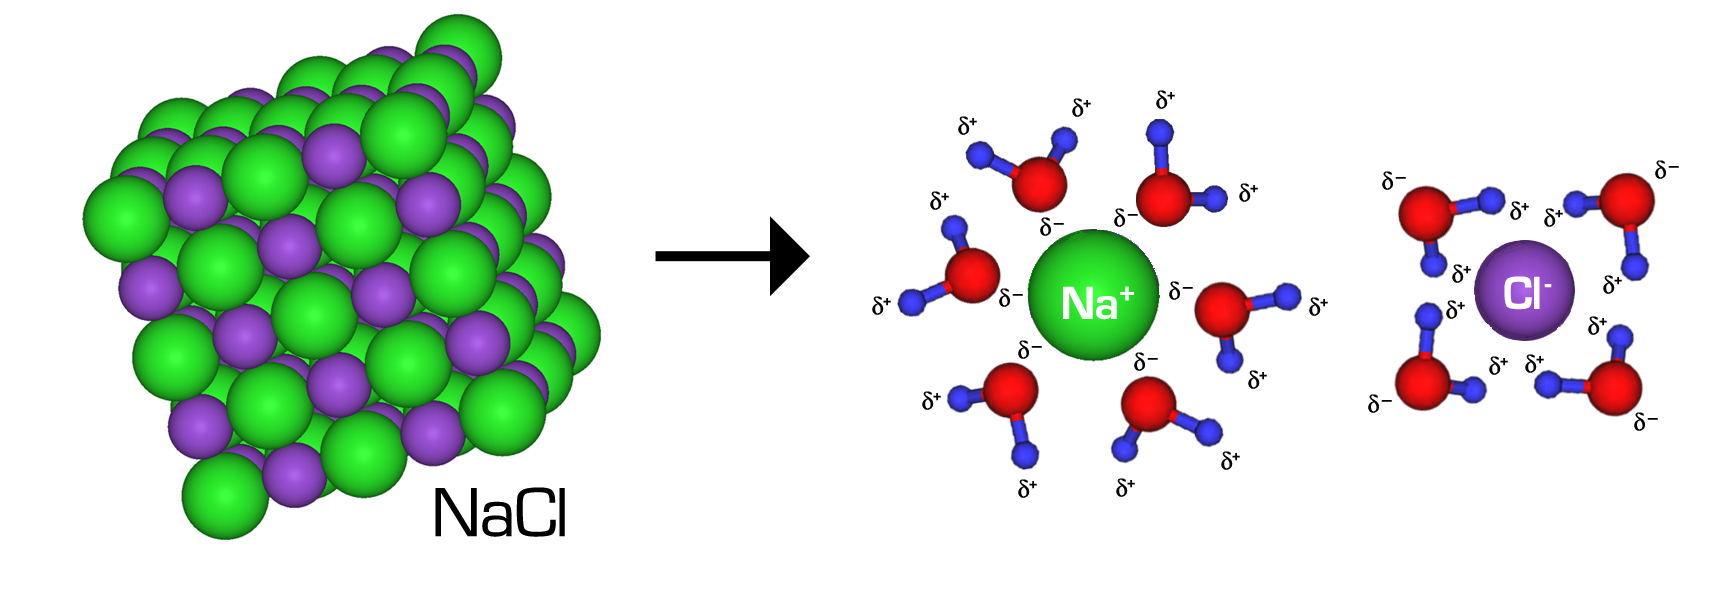
\includegraphics[height=4cm]{Images/anhhoa11/hoatanNaCl_2.jpg}
		\captionof{figure}{Quá trình điện li NaCl trong nước}
	\end{center}
\end{hopvidu}
\subsubsection{Thuyết acid-base của bronsted - lowry}
\Noibat[\maunhan]{Khái niệm acid và base theo bronsted - lowry}
%%%==============Bai_BT1==============%%%
\begin{hoivadap}
	\begin{cauhoi}
		Cho các dung dịch: $\mathrm{HCl}, \mathrm{NaOH}, \mathrm{Na_2CO_3}$.
		\begin{enumerate}
			\item Viết phương trình điện li của các chất trên.
			\item Theo khái niệm acid-base trong môn Khoa học tự nhiên ở lớp 8, trong những chất cho ở trên: Chất nào là acid? Chất nào là base?
			\item Sử dụng máy đo pH (hoặc giấy pH) xác định pH, môi trường (acid/base) của các dung dịch trên.
		\end{enumerate}
	\end{cauhoi}
	\loigiai{
		\begin{enumerate}
			\item Phương trình điện li của các chất:
			\[
			\mathrm{HCl} \rightarrow \mathrm{H}^+ + \mathrm{Cl}^-
			\]
			\[
			\mathrm{NaOH} \rightarrow \mathrm{Na}^+ + \mathrm{OH}^-
			\]
			\[
			\mathrm{Na_2CO_3} \rightarrow 2\mathrm{Na}^+ + \mathrm{CO_3}^{2-}
			\]
			\item Theo khái niệm acid-base trong môn Khoa học tự nhiên ở lớp 8:
			\begin{itemize}
				\item HCl là acid vì nó giải phóng ion H\(^+\) khi hòa tan trong nước.
				\item NaOH là base vì nó giải phóng ion OH\(^-\) khi hòa tan trong nước.
				\item Na\(_2\)CO\(_3\) không phải là bazơ vì khi tan vào nước nó không phân ly ra $OH^-$.
			\end{itemize}
			\item Sử dụng máy đo pH (hoặc giấy pH) xác định:
			\begin{itemize}
				\item Dung dịch HCl: pH < 7, môi trường acid.
				\item Dung dịch NaOH: pH > 7, môi trường base.
				\item Dung dịch Na\(_2\)CO\(_3\): pH > 7, môi trường base.
			\end{itemize}
	\end{enumerate}}
\end{hoivadap}
\begin{hoivadap}
	\begin{cauhoi}
	Nếu theo quan điểm cũ, Na\(_2\)CO\(_3\) không phải là bazơ vì không phân ly ra ion OH\(^-\). Tuy nhiên, khi đo pH, ta lại thấy dung dịch Na\(_2\)CO\(_3\) có tính bazơ. Điều này có mâu thuẫn không?
	\end{cauhoi}
	\loigiai{Khái niệm acid-base đề cập ở lớp 8 chỉ đúng với dung môi nước và chưa phản ánh đầy đủ bản chất acid/base. Năm 1923, nhà hoá học người Đan Mạch J. Brønsted (Bronstết) và nhà hoá học người Anh T. Lowry (Lao-ri) đã đưa ra một định nghĩa tổng quát hơn về acid, base.}
\end{hoivadap}
\vspace{0.25cm}
\begin{tomtat}
	\indam{Thuyết Brønsted - Lowry:} \indam[\mauphu]{acid} là chất \indam[\mauphu]{cho proton} $\left(\mathrm{H}^{+}\right)$ và \indam[\mauphu]{base} là chất \indam[\mauphu]{nhận proton}. Acid và base có thể là phân tử hoặc ion.
\end{tomtat}

\begin{vidu}
	\begin{enumerate}
		\item \begin{tikzpicture}[anchor=base, baseline]
		\tikzstyle{mynode} =[
		font=\bfseries,
		anchor=base,
		align =center,
		minimum width = 1cm,
		minimum height = .65cm
		]
		%%%==================%%%
		\tikzstyle{mymatrix} = [
		matrix of nodes,
		nodes in empty cells,
		nodes={mynode},
		column sep=-\pgflinewidth,
		row sep = -\pgflinewidth
		]
		%%%=======================================================%%%
		\matrix(m) [mymatrix]{
		$\mathsf{\color{\maunhan}HCl}$	& + & $\mathsf{H_2O}$ & $\xleftrightarrow$ & $\mathsf{\color{\maunhan}H_3O^+}$ &  + & $\mathsf{Cl^-}$\\
		};
		\path [draw,-stealth,line width=1pt] ([xshift=-0.25cm]m-1-1.south) |-([yshift=-0.5cm]m-1-2.south)node[above]{$H^+$}-|(m-1-3.south) ;
	\end{tikzpicture}
	\\
	Trong phản ứng trên: HCl cho $\mathrm{H}^{+}, \mathrm{HCl}$ là acid; $\mathrm{H}_2 \mathrm{O}$ nhận $\mathrm{H}^{+}, \mathrm{H}_2 \mathrm{O}$ là base.
	%%%
	\item \begin{tikzpicture}[anchor=base, baseline]
		\tikzstyle{mynode} =[
		font=\bfseries,
		anchor=base,
		align =center,
		minimum width = 1cm,
		minimum height = .65cm
		]
		%%%==================%%%
		\tikzstyle{mymatrix} = [
		matrix of nodes,
		nodes in empty cells,
		nodes={mynode},
		column sep=-\pgflinewidth,
		row sep = -\pgflinewidth
		]
		%%%=======================================================%%%
		\matrix(m) [mymatrix]{
			$\mathsf{NH_3}$	& + & $\mathsf{\color{\maunhan}H_2O}$ & $\xleftrightarrow$ & $\mathsf{\color{\maunhan}NH_4^+}$ &  + & $\mathsf{OH^-}$\\
		};
		\path [draw,<-,line width=1pt,>=stealth] ([xshift=-0.25cm]m-1-1.south) |-([yshift=-0.5cm]m-1-2.south)node[above,xshift=-0.25cm]{$H^+$}-|([xshift=-0.25cm]m-1-3.south) ;
	\end{tikzpicture}
	\\
	Trong phản ứng trên: $H_2O$ cho $\mathrm{H}^{+}, \mathrm{H_2O}$ là acid; $\mathrm{NH}_3$ nhận $\mathrm{H}^{+}$, $\mathrm{NH}_3$ là base.
	%%%
		%%%
	\item \begin{tikzpicture}[anchor=base, baseline]
		\tikzstyle{mynode} =[
		font=\bfseries,
		anchor=base,
		align =center,
		minimum width = 1cm,
		minimum height = .65cm
		]
		%%%==================%%%
		\tikzstyle{mymatrix} = [
		matrix of nodes,
		nodes in empty cells,
		nodes={mynode},
		column sep=-\pgflinewidth,
		row sep = -\pgflinewidth
		]
		%%%=======================================================%%%
		\matrix(m) [mymatrix]{
			$\mathsf{CO_3^{2-}}$	& + & $\mathsf{\color{\maunhan}H_2O}$ & $\xleftrightarrow$ & $\mathsf{\color{\maunhan}HCO_3^-}$ &  + & $\mathsf{OH^-}$\\
		};
		\path [draw,<-,line width=1pt,>=stealth] ([xshift=-0.25cm]m-1-1.south) |-([yshift=-0.5cm]m-1-2.south)node[above,xshift=-0.25cm]{$H^+$}-|([xshift=-0.25cm]m-1-3.south) ;
		\path [draw,->,line width=1pt,>=stealth] ([xshift=-0.45cm]m-1-5.north) |-([yshift=0.5cm]m-1-6.north)node[below,xshift=-0.35cm]{$H^+$}-|([xshift=-0.25cm]m-1-7.north) ;
	\end{tikzpicture}
	\\
	Trong phản ứng thuận, $\mathrm{CO}_3^{2-}$ nhận $\mathrm{H}^{+}$của $\mathrm{H}_2 \mathrm{O}, \mathrm{CO}_3^{2-}$ là base, $\mathrm{H}_2 \mathrm{O}$ là acid. Trong phản ứng nghịch, ion $\mathrm{HCO}_3^{-}$là acid, ion $\mathrm{OH}^{-}$là base.
	\end{enumerate}
\end{vidu}
%%%==============Bai_BT1==============%%%
\begin{hoivadap}
	\begin{cauhoi}
		Dựa vào thuyết acid-base của Brønsted-Lowry, hãy xác định chất nào là acid, chất nào là base trong các phản ứng sau:
		\begin{enumerate}
			\item $\mathrm{CH_3COOH} + \mathrm{H_2O} \rightleftharpoons \mathrm{CH_3COO^{-}} + \mathrm{H_3O^{+}}$
			\item $\mathrm{S^{2-}} + \mathrm{H_2O} \rightleftharpoons \mathrm{HS^{-}} + \mathrm{OH^{-}}$
		\end{enumerate}
	\end{cauhoi}
	\loigiai{
		Dựa vào thuyết acid-base của Brønsted-Lowry, một acid là chất cho proton (H\(^+\)) và một base là chất nhận proton. Áp dụng định nghĩa này vào từng phản ứng:
		\begin{enumerate}
			\item $\mathrm{CH_3COOH} + \mathrm{H_2O} \rightleftharpoons \mathrm{CH_3COO^{-}} + \mathrm{H_3O^{+}}$
			\begin{itemize}
				\item $\mathrm{CH_3COOH}$ là acid vì nó cho proton (H\(^+\)) để tạo thành $\mathrm{CH_3COO^{-}}$.
				\item $\mathrm{H_2O}$ là base vì nó nhận proton (H\(^+\)) để tạo thành $\mathrm{H_3O^{+}}$.
			\end{itemize}
			\item $\mathrm{S^{2-}} + \mathrm{H_2O} \rightleftharpoons \mathrm{HS^{-}} + \mathrm{OH^{-}}$
			\begin{itemize}
				\item $\mathrm{S^{2-}}$ là base vì nó nhận proton (H\(^+\)) từ nước để tạo thành $\mathrm{HS^{-}}$.
				\item $\mathrm{H_2O}$ là acid vì nó cho proton (H\(^+\)) để tạo thành $\mathrm{OH^{-}}$.
			\end{itemize}
		\end{enumerate}
	}
\end{hoivadap}
\Noibat[\maunhan]{Ưu điểm của thuyết bronsted - lowry }
\vspace{0.25cm}
\begin{tomtat}
	Ưu điểm của thuyết acid-base Bronsted-Lowry so với thuyết Arrhenius:
	\begin{enumerate}
		\item  Phạm vi áp dụng rộng hơn: Thuyết Bronsted-Lowry không chỉ áp dụng cho các phản ứng trong dung dịch nước như thuyết Arrhenius, mà còn có thể áp dụng cho các phản ứng trong môi trường khác như dung dịch amoniac, dung dịch acid anhhydric, etc.
		\item  Định nghĩa acid-base cụ thể hơn: Theo Bronsted-Lowry, acid là chất cho proton (H+), base là chất nhận proton. Định nghĩa này rõ ràng hơn và bao quát hơn so với định nghĩa acid-base của Arrhenius chỉ dựa trên sự tan trong nước.
		\item  Phản ứng acid-base không chỉ xảy ra trong dung dịch, mà còn có thể xảy ra trong các chất rắn, khí.
		\item  Thuyết Bronsted-Lowry giải thích được nhiều hiện tượng mà thuyết Arrhenius không thể giải thích, như phản ứng tạo phức men-chất nền, phản ứng trao đổi prôton.
	\end{enumerate}
\end{tomtat}
\subsubsection{pH và chất chỉ thị acid - Base}
\Noibat[][][]{Tìm hiểu về pH}
\\
Nước là chất điện li yếu: 
\[
\mathrm{H}_2 \mathrm{O} \rightleftharpoons \mathrm{H}^{+}+\mathrm{OH}^{-}
\]
Tích số ion của nước, kí hiệu $\mathrm{K}_{\mathrm{w}}$ :
\begin{center}
	\boxct{$\mathrm{K}_{\mathrm{w}}=\left[\mathrm{H}^{+}\right]\left[\mathrm{OH}^{-}\right]$}
\end{center}
Ở $25^{\circ} \mathrm{C}, \mathrm{K}_{\mathrm{w}}=\left[\mathrm{H}^{+}\right]\left[\mathrm{OH}^{-}\right]=10^{-14}$. Đối với nước nguyên chất có $ [H^+] = [OH^-] =10^{-7}$.
\\
Nồng độ ion $\mathrm{H}^{+}$hoặc ion $\mathrm{OH}^{-}$được dùng để đánh giá tính acid hoặc tính base của các dung dịch. Tuy nhiên, nếu các dung dịch có nồng độ $\mathrm{H}^{+}$, nồng độ $\mathrm{OH}^{-}$thấp, chúng là những số có số mũ âm hoặc có nhiều chữ số thập phân. Vì vậy, để tiện sử dụng, người ta dùng đại lượng pH với quy ước như sau:
\[
\hopcttoan{\mathrm{pH}=-\lg \left[\mathrm{H}^{+}\right] \text {hoặc }\left[\mathrm{H}^{+}\right]=10^{-\mathrm{pH}}}
\]
Trong đó $\left[\mathrm{H}^{+}\right]$là nồng độ mol của ion $\mathrm{H}^{+}$.
Nếu dung dịch có $\left[\mathrm{H}^{+}\right]=10^{-\mathrm{a}} \mathrm{mol} / \mathrm{L}$ thì $\mathrm{pH}=\mathrm{a}$.
\begin{hopdongian}
	Dựa vào nồng độ $H^+$  có thể đánh giá môi trường của dung dịch
	\begin{enumerate}
		\item  Môi trường acid là môi trường có $\left[\mathrm{H}^{+}\right]>\left[\mathrm{OH}^{-}\right]$nên $\left[\mathrm{H}^{+}\right]>10^{-7}\mathrm{~mol}/\mathrm{L}$ hay $\mathrm{pH}<7$.
		\item  Môi trường base là môi trường có $\left[\mathrm{H}^{+}\right]<\left[\mathrm{OH}^{-}\right]$nên $\left[\mathrm{H}^{+}\right]<10^{-7}\mathrm{~mol}/\mathrm{L}$ hay $\mathrm{pH}>7$.
		\item  Môi trường trung tính là môi truờng có $\left[\mathrm{H}^{+}\right]=\left[\mathrm{OH}^{-}\right]=10^{-7} \mathrm{~mol}/\mathrm{L}$ hay $\mathrm{pH}=7$.
	\end{enumerate}
\end{hopdongian}
\noindent Thang pH thường dùng có giá trị từ 1 đến 14
	\begin{hopdongian}[\mauphu]
		\begin{center}
		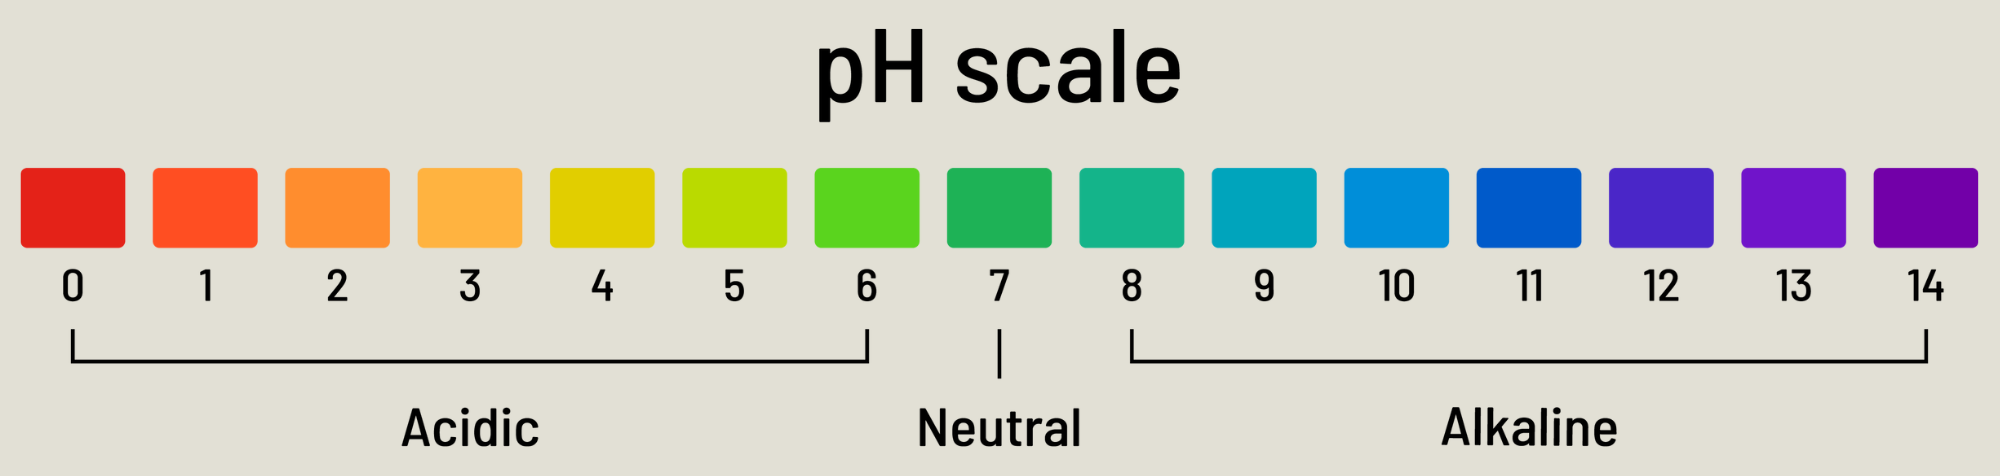
\includegraphics[width=12cm]{Images/anhhoa11/pHscale.png}
		\captionof{figure}{thang pH\label{fig:pHScale}}
		\end{center}
	\end{hopdongian}
\Noibat[][][]{Ý nghĩa pH trong thực tiễn}
\begin{tcolorbox}[
	enhanced jigsaw,
	frame hidden,
	colback=\mycolor!15,
	arc is angular,
	breakable
	]
	Thang đo pH là một công cụ quan trọng để duy trì sự cân bằng và an toàn trong nhiều lĩnh vực của cuộc sống hàng ngày.
\begin{enumerate}
	\item \indam{Kiểm soát chất lượng nước:}
	pH của nước ảnh hưởng đến sự sống của các sinh vật trong nước. Ví dụ, nước có pH quá thấp (acid) có thể gây hại cho cá và các sinh vật thủy sinh. Trong xử lý nước, kiểm tra và điều chỉnh pH là cần thiết để đảm bảo nước an toàn cho con người và động vật.
	\item \indam{Sản xuất thực phẩm và đồ uống:}
	 pH ảnh hưởng đến hương vị, màu sắc và độ an toàn của thực phẩm. Ví dụ, pH của rượu vang, sữa chua và pho mát phải được kiểm soát để đảm bảo chất lượng sản phẩm. Ngoài ra, trong ngành công nghiệp đồ uống, pH còn ảnh hưởng đến sự phát triển của vi khuẩn và quá trình lên men.
	\item \indam{Dược phẩm và y học:}
	pH có vai trò quan trọng trong việc hấp thu và hiệu quả của thuốc. Một số loại thuốc chỉ hoạt động tốt ở một mức pH nhất định, do đó việc điều chỉnh pH của môi trường là cần thiết để đảm bảo thuốc có tác dụng.
	\item \indam{Nông nghiệp:}
	 Đất có pH phù hợp là yếu tố quan trọng đối với sự phát triển của cây trồng. Đất có pH quá cao hoặc quá thấp có thể ảnh hưởng đến khả năng hấp thụ dinh dưỡng của cây. Nông dân thường kiểm tra pH của đất để điều chỉnh phân bón và cải tạo đất.
	\item \indam{Mỹ phẩm:}
	pH của các sản phẩm chăm sóc da và tóc ảnh hưởng đến tính an toàn và hiệu quả của chúng. Các sản phẩm như sữa rửa mặt, dầu gội, và kem dưỡng da cần có pH tương thích với da và tóc để tránh kích ứng và bảo vệ lớp màng acid tự nhiên.
	\item \indam{Xử lý chất thải:}
	pH của chất thải phải được kiểm soát trước khi xả ra môi trường để ngăn ngừa ô nhiễm. Nước thải công nghiệp thường phải được trung hòa pH trước khi xả ra hệ thống thoát nước hoặc sông ngòi.
\end{enumerate}
\end{tcolorbox}
\Noibat[][][]{Chất chỉ thị axit-base}
\vspace{0.5cm}
\begin{tomtat}
	Chất chỉ thị acid - base là chất có màu sắc biến đổi theo giá trị pH của dung dịch.\\
	Một số chất chỉ thị axit-bazo phổ biến:
	\begin{itemize}
		\item Quỳ tím Trong môi trường acid (pH < 7), quỳ tím chuyển sang màu đỏ.Trong môi trường base (pH > 7), quỳ tím chuyển sang màu xanh.
		\item  Phenolphthalein: Chuyển từ không màu (pH < 7) sang hồng (pH > 8.2).
		\item  Methyl orange: Chuyển từ đỏ (pH < 3.1) sang vàng (pH > 4.4).
		\item  Bromothymol blue: Chuyển từ vàng (pH < 6.0) sang xanh dương (pH > 7.6).
	\end{itemize}
\end{tomtat}
\begin{Bancobiet}
	\begin{center}
		\Large\indam{Mối quan hệ giữa pH và màu sắc của hoa cẩm tú cầu}
	\end{center}
	\vspace*{-0.5cm}
	\immini{Hoa cẩm tú cầu (Hydrangea) có thể thay đổi màu sắc dựa trên độ pH của đất nơi chúng được trồng. Sự thay đổi màu sắc chủ yếu được điều chỉnh bởi các hợp chất anthocyanins trong hoa và ion nhôm ($Al^{3+}$) trong đất. 
		\begin{itemize}
			\item Trong đất acid (pH dưới $6.0$): Hoa cẩm tú cầu thường có màu xanh dương.
			\item Trong đất trung tính (pH khoảng $6.0 - 7.0$): Hoa có thể có màu tím nhạt hoặc xanh dương nhạt. 
			\item Trong đất kiềm (pH trên $7.0$): Hoa cẩm tú cầu thường chuyển sang màu hồng hoặc đỏ. 
		\end{itemize}
		}{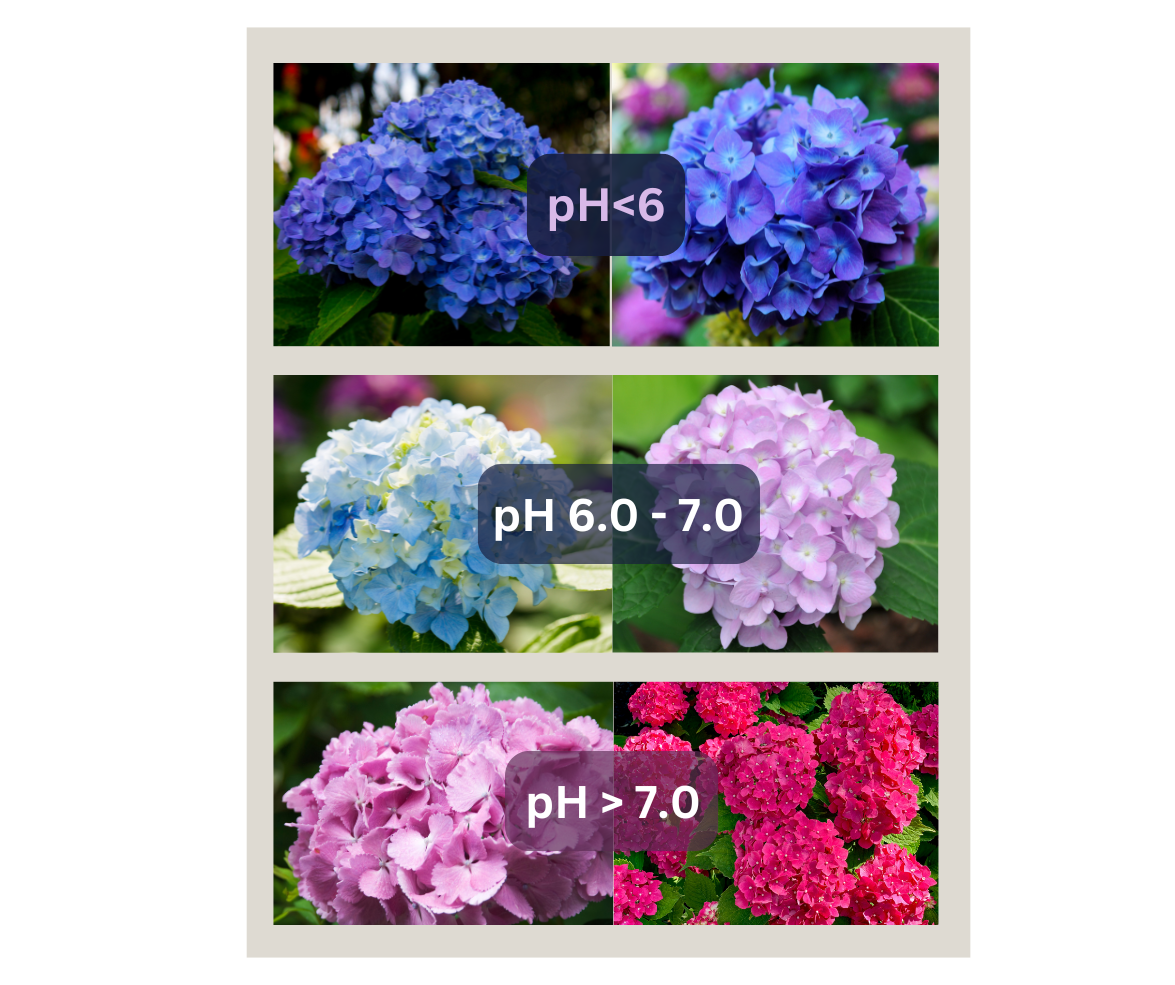
\includegraphics[height=7.5cm,trim={4.2cm 0cm 4.2cm 0cm},clip]{Images/anhhoa11/hoacamtucau.png}}
		Điều chỉnh độ pH của đất có thể giúp thay đổi màu sắc của hoa: thêm các vật liệu làm acid đất như nhôm sulfate để tạo màu xanh dương, hoặc thêm vôi nông nghiệp để làm tăng pH và tạo màu hồng. Các yếu tố khác như loại đất, tình trạng dinh dưỡng và lượng nước cũng ảnh hưởng đến màu sắc của hoa.
\end{Bancobiet}
\subsubsection{Sự thủy phân của muối}
Trong dung dịch nước, một số ion như $\mathrm{Al}^{3+}, \mathrm{Fe}^{3+}$ và $\mathrm{CO}_3^{2-}$ phản ứng với nước tạo ra các dung dịch có môi trường acid/base.
\begin{vidu}
	\begin{enumerate}
		\item Trong dung dịch $\mathrm{Na}_2 \mathrm{CO}_3$, ion $\mathrm{Na}^{+}$ không bị thủy phân, còn $\mathrm{CO}_3^{2-}$ thủy phân trong nước tạo ion $\mathrm{OH}^{-}$ theo phương trình:
		\[
		\mathrm{CO}_3^{2-}+\mathrm{H}_2 \mathrm{O} \rightleftharpoons \mathrm{HCO}_3^{-}+\mathrm{OH}^{-}
		\]
		Vì vậy, dung dịch $\mathrm{Na}_2 \mathrm{CO}_3$ có môi trường base.
		\item Trong dung dịch $\mathrm{AlCl}_3$ và $\mathrm{FeCl}_3$, ion $\mathrm{Cl}^{-}$không bị thuỷ phân, các ion $\mathrm{Al}^{3+}$ và $\mathrm{Fe}^{3+}$ bị thuỷ phân trong nước tạo ion $\mathrm{H}^{+}$theo phương trình ở dạng đơn giản như sau:
		\[
		\begin{aligned}
			& \mathrm{Al}^{3+}+\mathrm{H}_2 \mathrm{O} \rightleftharpoons \mathrm{Al}(\mathrm{OH})^{2+}+\mathrm{H}^{+} \\
			& \mathrm{Fe}^{3+}+\mathrm{H}_2 \mathrm{O} \rightleftharpoons \mathrm{Fe}(\mathrm{OH})^{2+}+\mathrm{H}^{+}
		\end{aligned}
		\]
		Do đó, dung dịch $\mathrm{AlCl}_3, \mathrm{FeCl}_3$ có môi trường acid. Trong thực tế, các loại đất có chứa nhiều ion $\mathrm{Al}^{3+}, \mathrm{Fe}^{3+}$ có giá trị pH thấp hay còn gọi là đất chua. Để khử chua, người ta bón vôi cho đất.
		
		Các muối nhôm và sắt, ví dụ: phèn nhôm $\left(\left(\mathrm{NH}_4\right)_2 \mathrm{SO}_4 \cdot \mathrm{Al}_2\left(\mathrm{SO}_4\right)_3 \cdot 24 \mathrm{H}_2 \mathrm{O}\right)$ và phèn sắt $\left(\left(\mathrm{NH}_4\right)_2 \mathrm{SO}_4 \cdot \mathrm{Fe}_2\left(\mathrm{SO}_4\right)_3 \cdot 24 \mathrm{H}_2 \mathrm{O}\right)$ được sử dụng làm chất keo tụ trong quá trình xử lí nước, dùng làm chất cầm màu trong công nghiệp dệt, nhuộm, hoặc làm chất kết dính, chống nhoè trong công nghiệp giấy,...
	\end{enumerate}
\end{vidu}
\subsubsection{Chuẩn độ acid -base}
Chuẩn độ là phương pháp xác định nồng độ của một chất bằng một dung dịch chuần đã biết nồng độ. Dựa vào thể tích của các dung dịch khi phản ứng vừa đủ với nhau, xác định được nồng độ dung dịch chất cần chuần độ.
\\
Trong phòng thí nghiệm, nồng độ của dung dịch base mạnh (ví dụ NaOH ) được xác định bằng một dung dịch acid mạnh (ví dụ HCl ) đã biết trước nồng độ mol dựa trên phản ứng:
\[
\mathrm{NaOH}+\mathrm{HCl} \longrightarrow \mathrm{NaCl}+\mathrm{H}_2 \mathrm{O}
\]
Khi các chất phản ứng vừa đủ với nhau, số mol HCl phản ứng bằng số mol NaOH .
Ta có:
\[
\mathrm{V}_{\mathrm{HCl}} \cdot \mathrm{C}_{\mathrm{HCl}}=\mathrm{V}_{\mathrm{NaOH}} \cdot \mathrm{C}_{\mathrm{NaOH}}
\]
Trong đó:
	\begin{itemize}
		\item $\mathrm{C}_{\mathrm{HCl}}$ và $\mathrm{C}_{\mathrm{NaOH}}$ lần lượt là nồng độ mol của dung dịch HCl và dung dịch NaOH ;
		\item $\mathrm{V}_{\mathrm{HCl}}$ và $\mathrm{V}_{\mathrm{NaOH}}$ lần lượt là thể tích của dung dịch HCl và dung dịch NaOH (cùng đơn vị đo).
	\end{itemize}
Khi biết $\mathrm{V}_{\mathrm{HCl}}, \mathrm{V}_{\mathrm{NaOH}}$ trong quá trình chuẩn độ và biết $\mathrm{C}_{\mathrm{HCl}}$ sẽ tính được $\mathrm{C}_{\mathrm{NaOH}}$.\\
Thời điểm để kết thúc chuẩn độ được xác định bằng sự đổi màu của chất chỉ thị phenolphthalein.
\subsection{Các dạng bài tập}
\begin{dang}{Câu hỏi lý thuyết}
\end{dang}
%%%=============Ví dụ mấu dạng 1=================%%%
\Noibat[][][\faBookmark]{Ví dụ mẫu}
%%%==============VDM1==============%%%
\begin{vd}
	Chất nào sau đây là chất điện ly?
	\choice
	{Đường saccharose}
	{Ethanol}
	{\True Natri clorua}
	{Dầu hỏa}
	\loigiai{Natri clorua (NaCl) là một chất điện ly vì nó phân ly thành các ion $Na^+$ và $Cl^-$ khi hòa tan trong nước. Các chất còn lại như đường saccharose, ethanol và dầu hỏa không phân ly thành ion trong dung dịch nước, do đó không phải là chất điện ly.}
\end{vd}
%%%=============EX_2=============%%%
\begin{vd}
	Theo thuyết Brønsted-Lowry, acid là chất:
	\choice
	{Nhận proton}
	{\True Cho proton}
	{Nhận electron}
	{Cho electron}
	\loigiai{Theo thuyết Brønsted-Lowry, acid được định nghĩa là chất cho proton $(H^+)$. Base, ngược lại, là chất nhận proton. Định nghĩa này khác với thuyết Lewis về acid-base, trong đó acid được xem là chất nhận cặp electron và base là chất cho cặp electron.}
\end{vd}
%%%%=============EX_3=============%%%
%%%==============HetVDM1==============%%%
\Noibat[][][\faBank]{Bài tập tự luyện dạng \thedang}

%%%=============SOẠN EX===============%%%
\Opensolutionfile{ansex}[Ans/LGEX-H11C01B02-BTTL01]
\Opensolutionfile{ans}[Ans/Ans-H11C01B02-BTTL01]
%\tatloigiaiex
%\luuloigiaiex
%%%=========ex_1=========%%%
%%%=============EX_1=============%%%
\begin{ex}
	Giá trị pH của máu người khỏe mạnh thường nằm trong khoảng:
	\choice
	{$4{,}5-6{,}5$}
	{$6{,}5-7{,}0$}
	{\True $7{,}35-7{,}45$}
	{$8{,}0-9{,}0$}
	\loigiai{Máu của người khỏe mạnh có pH nằm trong khoảng hẹp từ $7{,}35$ đến $7{,}45$. Đây là một khoảng pH hơi kiềm nhẹ, rất quan trọng cho sự hoạt động bình thường của các enzyme và protein trong cơ thể. Sự thay đổi nhỏ trong pH máu có thể dẫn đến các vấn đề sức khỏe nghiêm trọng.}
\end{ex}
%%%=============EX_4=============%%%
\begin{ex}
	Chất chỉ thị nào sau đây chuyển màu từ không màu sang hồng trong môi trường kiềm?
	\choice
	{Quỳ tím}
	{Methyl da cam}
	{\True Phenolphthalein}
	{Bromothymol blue}
	\loigiai{Phenolphthalein là một chất chỉ thị acid-base phổ biến, không màu trong môi trường acid và trung tính (pH $<8{,}2)$ và chuyển sang màu hồng trong môi trường kiềm (pH $>8{,}2)$. Đặc tính này làm cho phenolphthalein trở thành một chất chỉ thị hữu ích trong các phép chuẩn độ acid-base, đặc biệt khi chuẩn độ acid yếu bằng base mạnh.}
\end{ex}

%%%=============EX_6=============%%%
\begin{ex}
	Trong dung dịch nước, ion $\mathrm{Al}^{3+}$ tồn tại dưới dạng cân bằng:
	\choice
	{$\mathrm{Al}^{3+} + 3\mathrm{H}_2\mathrm{O} \rightleftharpoons \mathrm{Al(OH)}_3 + 3\mathrm{H}^+$}
	{$\mathrm{Al}^{3+} + 2\mathrm{H}_2\mathrm{O} \rightleftharpoons \mathrm{Al(OH)}_2^+ + 2\mathrm{H}^+$}
	{\True $\mathrm{Al}^{3+} + \mathrm{H}_2\mathrm{O} \rightleftharpoons \mathrm{Al(OH)}^{2+} + \mathrm{H}^+$}
	{$\mathrm{Al}^{3+} + 4\mathrm{H}_2\mathrm{O} \rightleftharpoons \mathrm{Al(OH)}_4^- + 4\mathrm{H}^+$}
	\loigiai{Trong dung dịch nước, ion $\mathrm{Al}^{3+}$ tham gia vào phản ứng thủy phân, tạo ra cân bằng với ion $\mathrm{Al(OH)}^{2+}$. Phương trình cân bằng chính xác là $\mathrm{Al}^{3+} + \mathrm{H}_2\mathrm{O} \rightleftharpoons \mathrm{Al(OH)}^{2+} + \mathrm{H}^+$. Đây là bước đầu tiên trong quá trình thủy phân của $\mathrm{Al}^{3+}$, và là cân bằng chủ yếu trong dung dịch nước.}
\end{ex}
%%%$=============EX_7=============$%%%
\begin{ex}
	Giá trị pH của một dung dịch acid mạnh $0{,}001M$ là:
	\choice
	{$1$}
	{$2$}
	{\True $3$}
	{$4$}
	\loigiai{Đối với acid mạnh, ta giả định rằng nó phân ly hoàn toàn trong nước. Với nồng độ $0{,}001M$, nồng độ ion $H+$ sẽ bằng $0{,}001M$.
		Áp dụng công thức pH $= -log[H+]$, ta có:
		pH $=-log(0{,}001)= -log(10^-3)=3$
		Vì vậy, giá trị pH của dung dịch acid mạnh $0{,}001M$ là $3$.}
\end{ex}
%%%$=============EX_8=============$%%%
\begin{ex}
	Trong phản ứng: $\mathrm{NH}_3 + \mathrm{H}_2\mathrm{O} \rightleftharpoons \mathrm{NH}_4^+ + \mathrm{OH}^-$, theo thuyết Brønsted-Lowry, $\mathrm{NH}_3$ đóng vai trò là:
	\choice
	{Acid}
	{\True Base}
	{Vừa acid vừa base}
	{Không phải acid cũng không phải base}
	\loigiai{Trong phản ứng này, $\mathrm{NH}_3$ (amoniac) nhận một proton $(H+)$ từ $\mathrm{H}_2\mathrm{O}$ để tạo thành $\mathrm{NH}_4^+$. Theo thuyết Brønsted-Lowry, chất nhận proton được định nghĩa là base. Do đó, trong phản ứng này, $\mathrm{NH}_3$ đóng vai trò là base Brønsted-Lowry.}
\end{ex}
%%%$=============EX_9=============$%%%
\begin{ex}
	Quỳ tím chuyển sang màu gì khi nhúng vào dung dịch có pH $=3$?
	\choice
	{Xanh}
	{\True Đỏ}
	{Tím}
	{Không đổi màu}
	\loigiai{Quỳ tím là một chất chỉ thị acid-base phổ biến. Nó có màu tím ở pH trung tính (khoảng $7$), chuyển sang màu đỏ trong môi trường acid (pH $<7)$ và màu xanh trong môi trường kiềm (pH $>7)$. Với pH $=3$, dung dịch có tính acid mạnh, do đó quỳ tím sẽ chuyển sang màu đỏ.}
\end{ex}
%%%%=============EX_10=============%%%
\begin{ex}
	Trong chuẩn độ acid-base, để xác định chính xác điểm tương đương, nên chọn chất chỉ thị có khoảng đổi màu:
	\choice
	{Trùng với pH tại điểm tương đương}
	{Cao hơn nhiều so với pH tại điểm tương đương}
	{Thấp hơn nhiều so với pH tại điểm tương đương}
	{\True Gần với pH tại điểm tương đương}
	\loigiai{Để xác định chính xác điểm tương đương trong chuẩn độ acid-base, nên chọn chất chỉ thị có khoảng đổi màu gần với pH tại điểm tương đương. Điều này đảm bảo rằng sự thay đổi màu sắc của chất chỉ thị xảy ra càng gần với điểm tương đương thực tế càng tốt, giúp tăng độ chính xác của phép chuẩn độ. Nếu khoảng đổi màu quá cao hoặc quá thấp so với pH tại điểm tương đương, có thể dẫn đến sai số đáng kể trong kết quả chuẩn độ.}
\end{ex}
%%%$=============EX_11=============$%%%
\begin{ex}
	Chất nào sau đây là chất điện ly?
	\choice
	{Đường saccharose}
	{Dầu hỏa}
	{\True Natri clorua}
	{Cồn ethylic nguyên chất}
	\loigiai{Natri clorua (NaCl) là một chất điện ly, khi hòa tan trong nước nó sẽ phân ly thành các ion $Na^+$ và $Cl^-$. Các chất còn lại không phân ly thành ion trong dung dịch nên không phải là chất điện ly.}
\end{ex}
%%%$=============EX_12=============$%%%
\begin{ex}
	Theo thuyết Brønsted - Lowry, acid là chất:
	\choice
	{Nhận proton}
	{\True Cho proton}
	{Nhận electron}
	{Cho electron}
	\loigiai{Theo thuyết Brønsted - Lowry, acid được định nghĩa là chất có khả năng cho proton $H^+$ trong phản ứng. Base là chất có khả năng nhận proton.}
\end{ex}
%%%$=============EX_13=============$%%%
\begin{ex}
	pH của một dung dịch trung tính ở $25\circ C$ là:
	\choice
	{$0$}
	{$14$}
	{\True $7$}
	{$1$}
	\loigiai{Ở $25\circ C$, một dung dịch được coi là trung tính khi có pH $=7$. Khi pH $<7$, dung dịch là acid; khi pH $>7$, dung dịch là base.}
\end{ex}
%%%$=============EX_14=============$%%%
\begin{ex}
	Công thức tính pH của dung dịch acid mạnh là:
	\choice
	{pH $= -log[OH_-]$}
	{pH $=14+ log[H+]$}
	{\True $pH = -log[H^+]$}
	{pH $= log[H^+]$}
	\loigiai{Công thức tính pH của dung dịch acid mạnh là $pH = -log[H+]$, trong đó $[H^+]$ là nồng độ ion hydro trong dung dịch.}
\end{ex}
%%%=============EX_15=============%%%
\begin{ex}
	Chất chỉ thị nào sau đây chuyển màu trong môi trường base?
	\choice
	{Methyl cam}
	{Methyl đỏ}
	{\True Phenolphthalein}
	{Xanh bromothymol}
	\loigiai{Phenolphthalein là chất chỉ thị chuyển màu trong môi trường base. Nó không màu trong môi trường acid và chuyển sang màu hồng trong môi trường base.}
\end{ex}
%%%=============EX_16=============%%%
\begin{ex}
	Trong phương pháp chuẩn độ acid - base, điểm tương đương là điểm mà:
	\choice
	{pH của dung dịch bằng 7}
	{Chất chỉ thị chuyển màu}
	{\True Số mol acid đã phản ứng hết với số mol base}
	{Thể tích dung dịch chuẩn độ bằng thể tích dung dịch được chuẩn độ}
	\loigiai{Điểm tương đương trong chuẩn độ acid - base là điểm mà số mol acid đã phản ứng hết với số mol base, tức là tại điểm này, lượng acid và base đã phản ứng với nhau theo tỉ lệ phản ứng hóa học.}
\end{ex}
%%%=============EX_17=============%%%
\begin{ex}
	Ion Al3+ trong dung dịch nước có tính:
	\choice
	{Trung tính}
	{Base}
	{\True Acid}
	{Lưỡng tính}
	\loigiai{Ion $Al^3+$ trong dung dịch nước có tính acid. Nó có thể tham gia phản ứng thủy phân tạo ra ion H+, làm tăng nồng độ H+ trong dung dịch: $Al^{3+}+ + H_2O \xrightleftharpoons Al(OH)^{2+} + H^+$}
\end{ex}
%%%=============EX_18=============%%%
\begin{ex}
	Quỳ tím chuyển màu gì trong môi trường acid?
	\choice
	{Xanh}
	{\True Đỏ}
	{Tím}
	{Không màu}
	\loigiai{Quỳ tím chuyển sang màu đỏ trong môi trường acid. Trong môi trường base, nó chuyển sang màu xanh, còn trong môi trường trung tính, nó giữ nguyên màu tím.}
\end{ex}
%%%=============EX_19=============%%%
\begin{ex}
	Phản ứng nào sau đây thể hiện tính chất của acid theo Brønsted - Lowry?
	\choice
	{$NaOH + HCl \rightarrow NaCl + H2O$}
	{$2Na + 2H_2O \rightarrow 2NaOH + H_2$}
	{\True $HCl + H_2O \rightarrow H_3O+ + Cl-$}
	{$CuO + 2HCl \rightarrow CuCl_2 + H_2O$}
	\loigiai{Phản ứng $HCl + H_2O → H_3O^+ + Cl^-$ thể hiện tính chất của acid theo Brønsted - Lowry. Trong phản ứng này, HCl đóng vai trò là acid (cho proton) và $H_2O$ đóng vai trò là base (nhận proton).}
\end{ex}
%%%=============EX_20=============%%%
\begin{ex}
	pH của máu người khỏe mạnh thường nằm trong khoảng:
	\choice
	{$4{,}5-5{,}5$}
	{$6{,}0-7{,}0$}
	{\True $7{,}35-7{,}45$}
	{$8{,}0-9{,}0$}
	\loigiai{pH của máu người khỏe mạnh thường nằm trong khoảng $7{,}35-7{,}45$. Đây là một khoảng pH hẹp và rất quan trọng cho sự hoạt động bình thường của các enzyme và quá trình trao đổi chất trong cơ thể.}
\end{ex}
%%%=============EX_21=============%%%
\begin{ex}
	Chất nào sau đây không phải là chất điện ly?
	\choice
	{NaCl}
	{$H_2SO_4$}
	{KOH}
	{\True $C_6H_{12}O_6$ (glucose)}
	\loigiai{$C_6H_{12}O_6$ (glucose) không phải là chất điện ly. Khi hòa tan trong nước, glucose không phân ly thành ion mà tồn tại dưới dạng phân tử. Các chất còn lại (NaCl, $H_2SO_4$, KOH) đều là chất điện ly, phân ly thành ion khi hòa tan trong nước.}
\end{ex}
%%%=============EX_22=============%%%
\begin{ex}
	Theo thuyết Brønsted - Lowry, trong phản ứng $NH3 + H2O \xrightleftharpoons{} NH4+ + OH-$, $NH_3$ đóng vai trò là:
	\choice
	{Acid}
	{\True Base}
	{Chất oxi hóa}
	{Chất khử}
	\loigiai{Trong phản ứng $NH3 + H2O \xrightleftharpoons{} NH4+ + OH-$, $NH_3$ đóng vai trò là base theo thuyết Brønsted - Lowry vì nó nhận proton ($H^+$) từ $H_2O$ để tạo thành $NH_4^+$. $H_2O$ trong trường hợp này đóng vai trò là acid, cho proton.}
\end{ex}
%%%=============EX_23=============%%%
\begin{ex}
	pH của nước cất tinh khiết ở $25^\circ C$ là:
	\choice
	{$0$}
	{$14$}
	{\True $7$}
	{$1$}
	\loigiai{pH của nước cất tinh khiết ở $25^\circ C$ là 7. Ở nhiệt độ này, nồng độ ion $H^+$ và $OH^-$ trong nước tinh khiết đều bằng $10^{-7} mol/L$, do đó $pH = -log[H+] = -log(10^{-7}) = 7$.}
\end{ex}
%%%=============EX_24=============%%%
\begin{ex}
	Công thức tính pOH của một dung dịch là:
	\choice
	{$pOH = -log[H^+]$}
	{$pOH = 14 + log[OH^-]$}
	{\True $pOH = -log[OH^-]$}
	{$pOH = log[OH^-]$}
	\loigiai{Công thức tính pOH của một dung dịch là $pOH = -log[OH^-]$, trong đó $[OH^-]$ là nồng độ ion hydroxide trong dung dịch. Chú ý rằng $pH + pOH = 14$ ở $25^\circ C$.}
\end{ex}
%%%=============EX_25=============%%%
\begin{ex}
	Chất chỉ thị nào sau đây chuyển màu trong khoảng pH từ $8{,}2$ đến $10$?
	\choice
	{Methyl cam}
	{Methyl đỏ}
	{\True Phenolphthalein}
	{Xanh bromothymol}
	\loigiai{Phenolphthalein là chất chỉ thị chuyển màu trong khoảng pH từ $8{,}2$ đến $10$. Nó không màu khi pH $<8{,}2$ và chuyển sang màu hồng khi pH $>8{,}2$.}
\end{ex}
%%%=============EX_26=============%%%
\begin{ex}
	Trong phương pháp chuẩn độ acid - base, điểm kết thúc chuẩn độ là:
	\choice
	{Điểm mà số mol acid bằng số mol base}
	{\True Điểm mà chất chỉ thị chuyển màu}
	{Điểm mà pH của dung dịch bằng 7}
	{Điểm mà thể tích dung dịch chuẩn độ bằng thể tích dung dịch được chuẩn độ}
	\loigiai{Điểm kết thúc chuẩn độ là điểm mà chất chỉ thị chuyển màu. Đây là điểm mà người thực hiện chuẩn độ quan sát được và dừng việc thêm dung dịch chuẩn độ. Điểm này thường gần với điểm tương đương nhưng không nhất thiết trùng khớp.}
\end{ex}
%%%=============EX_27=============%%%
\begin{ex}
	Ion Fe3+ trong dung dịch nước có tính:
	\choice
	{Trung tính}
	{Base}
	{\True Acid}
	{Lưỡng tính}
	\loigiai{Ion Fe3+ trong dung dịch nước có tính acid. Nó tham gia phản ứng thủy phân tạo ra ion H+, làm tăng nồng độ H+ trong dung dịch: $Fe^{3+} + H_2O \xrightleftharpoons{} Fe(OH)_2+ + H^+$}
\end{ex}
%%%=============EX_28=============%%%
\begin{ex}
	Giấy quỳ đỏ chuyển màu gì trong môi trường base?
	\choice
	{Đỏ}
	{\True Xanh}
	{Tím}
	{Không màu}
	\loigiai{Giấy quỳ đỏ chuyển sang màu xanh trong môi trường base. Trong môi trường acid, nó giữ nguyên màu đỏ.}
\end{ex}
%%%=============EX_29=============%%%
\begin{ex}
	Phản ứng nào sau đây thể hiện tính chất của base theo Brønsted - Lowry?
	\choice
	{$NaOH + HCl \xrightarrow{} NaCl + H_2O$}
	{$2Na + 2H_2O \xrightarrow{} 2NaOH + H_2$}
	{\True $NH_3 + H_2O \xrightleftharpoons{} NH_4^+ + OH^-$}
	{$CuO + 2HCl \xrightarrow{} CuCl_2 + H_2O$}
	\loigiai{Phản ứng $NH3 + H_2O \xrightleftharpoons{} NH_4^+ + OH^-$ thể hiện tính chất của base theo Brønsted - Lowry. Trong phản ứng này, NH3 đóng vai trò là base (nhận proton) và H2O đóng vai trò là acid (cho proton).}
\end{ex}
%%%=============EX_30=============%%%
\begin{ex}
	pH của nước mưa tự nhiên thường nằm trong khoảng:
	\choice
	{$1 - 2$}
	{\True $5{,}6 - 6{,}5$}
	{$7{,}0 - 8{,}0$}
	{$9{,}0 - 10{,}0$}
	\loigiai{pH của nước mưa tự nhiên thường nằm trong khoảng $5{,}6 - 6{,}5$. Nước mưa có tính acid nhẹ do hòa tan $CO_2$ từ không khí tạo thành acid carbonic ($H_2CO_3$).}
\end{ex}
%%%%=============EX_31=============%%%
\begin{ex}
	Dung dịch nào sau đây có $pH < 7$?
	\choice
	{Dung dịch NaOH}
	{Dung dịch $Na_2CO_3$}
	{\True Dung dịch HCl}
	{Dung dịch $NH_3$}
	\loigiai{Dung dịch HCl có $pH < 7$ vì HCl là một acid mạnh. Khi hòa tan trong nước, nó phân ly hoàn toàn tạo ra ion H+, làm tăng nồng độ $H^+$ trong dung dịch, dẫn đến $pH < 7$.}
\end{ex}
%%%=============EX_32=============%%%
\begin{ex}
	Trong phương trình $pH + pOH = 14$ (ở $25^\circ C$), 14 là giá trị của:
	\choice
	{pH của nước tinh khiết}
	{pOH của nước tinh khiết}
	{\True pKw (hằng số phân ly của nước)}
	{Nồng độ ion $H^+$ trong nước tinh khiết}
	\loigiai{Trong phương trình $pH + pOH = 14$ (ở $25^\circ C$), 14 là giá trị của pKw - hằng số phân ly của nước. Kw là tích ion của nước ($Kw = [H+][OH-] = 10^-14$ ở $25^\circ C$), và $pKw = -logKw = 14$.}
\end{ex}
%%%=============EX_33=============%%%
\begin{ex}
	Ion $CO_3^{2-}$ trong dung dịch nước có tính:
	\choice
	{Acid}
	{\True Base}
	{Trung tính}
	{Lưỡng tính}
	\loigiai{Ion $CO_3^{2-}$ trong dung dịch nước có tính base. Nó tham gia phản ứng thủy phân tạo ra ion $OH^-$, làm tăng nồng độ $OH^-$ trong dung dịch: $CO_3^{2-} + H_2O \xrightleftharpoons{} HCO_3^- + OH^-$}
\end{ex}
%%%=============EX_34=============%%%
\begin{ex}
	Trong phản ứng chuẩn độ giữa NaOH và HCl, chất chỉ thị nào sau đây phù hợp nhất?
	\choice
	{Phenolphthalein}
	{\True Methyl cam}
	{Xanh bromothymol}
	{Phenol đỏ}
	\loigiai{Methyl cam là chất chỉ thị phù hợp nhất cho phản ứng chuẩn độ giữa NaOH và HCl. Nó có khoảng chuyển màu từ pH $3{,}1$ đến $4{,}4$, gần với điểm tương đương của phản ứng giữa acid mạnh và base mạnh (pH khoảng $7$).}
\end{ex}
%%%=============EX_35=============%%%
\begin{ex}
	Nếu pH của một dung dịch là 4, thì pOH của dung dịch đó là bao nhiêu (ở 25°C)?
	\choice
	{4}
	{7}
	{\True 10}
	{14}
	\loigiai{Ở $25^\circ C$, ta có $pH + pOH = 14$. Nếu $pH = 4$, thì $pOH = 14 - pH = 14 - 4 = 10$.}
\end{ex}
%%%=============EX_36=============%%%
\begin{ex}
	Trong phản ứng $Al(OH)_3 + 3H+ \xrightleftharpoons{} Al3+ + 3H2O$, Al(OH)3 đóng vai trò là:
	\choice
	{Acid}
	{\True Base}
	{Chất oxi hóa}
	{Chất khử}
	\loigiai{Trong phản ứng $Al(OH)_3 + 3H^+ \xrightleftharpoons{} Al^{3+} + 3H_2O$, $Al(OH)_3$ đóng vai trò là base theo thuyết Brønsted - Lowry vì nó nhận proton $(H^+)$ từ acid.}
\end{ex}
%%%=============EX_37=============%%%
\begin{ex}
	Nồng độ ion H+ trong một dung dịch là $10^{-}3$ mol/L. pH của dung dịch này là:
	\choice
	{-3}
	{\True 3}
	{11}
	{13}
	\loigiai{$pH = -log[H+] = -log(10^-3) = 3$}
\end{ex}
%%%=============EX_38=============%%%
\begin{ex}
	Chất nào sau đây là chất lưỡng tính?
	\choice
	{NaOH}
	{HCl}
	{\True $Al(OH)_3$}
	{$H_2SO_4$}
	\loigiai{$Al(OH)_3$ là chất lưỡng tính. Nó có thể đóng vai trò là acid (cho proton) trong phản ứng với base mạnh, và đóng vai trò là base (nhận proton) trong phản ứng với acid mạnh.}
\end{ex}
%%%=============EX_39=============%%%
\begin{ex}
	Phương pháp chuẩn độ acid - base được sử dụng để xác định:
	\choice
	{Khối lượng riêng của acid hoặc base}
	{Nhiệt độ sôi của acid hoặc base}
	{\True Nồng độ của acid hoặc base}
	{Điện tích của ion trong dung dịch acid hoặc base}
	\loigiai{Phương pháp chuẩn độ acid - base được sử dụng để xác định nồng độ của acid hoặc base. Bằng cách sử dụng một dung dịch chuẩn đã biết nồng độ, ta có thể xác định được nồng độ chính xác của dung dịch acid hoặc base cần phân tích.}
\end{ex}
%%%=============EX_40=============%%%
\begin{ex}
	Trong phản ứng $NH_4^+ + OH^- \xrightleftharpoons{} NH_3 + H_2O$, $NH_4^+$ đóng vai trò là:
	\choice
	{\True Acid}
	{Base}
	{Chất oxi hóa}
	{Chất khử}
	\loigiai{Trong phản ứng $NH_4^+ + OH^- \xrightleftharpoons{} NH_3 + H_2O$, $NH_4^+$ đóng vai trò là acid theo thuyết Brønsted - Lowry vì nó cho proton ($H^+$) cho $OH^-$ để tạo thành H2O.}
\end{ex}
%%%%=============EX_41=============%%%
\begin{ex}
	pH của đất ảnh hưởng như thế nào đến sự phát triển của cây trồng?
	\choice
	{pH không ảnh hưởng đến sự phát triển của cây trồng}
	{Cây trồng phát triển tốt nhất ở pH rất thấp ($< 3$)}
	{Cây trồng phát triển tốt nhất ở pH rất cao ($> 10$)}
	{\True pH ảnh hưởng đến khả năng hấp thu dinh dưỡng của cây trồng}
	\loigiai{pH của đất ảnh hưởng đến khả năng hấp thu dinh dưỡng của cây trồng. Hầu hết các cây trồng phát triển tốt nhất ở pH từ $6{,}0$ đến $7{,}5$. Ở pH quá thấp hoặc quá cao, một số chất dinh dưỡng có thể trở nên không tan hoặc không sẵn có cho cây hấp thu.}
\end{ex}
%%%=============EX_42=============%%%
\begin{ex}
	Nồng độ ion $OH^-$ trong một dung dịch là $10^{-11}$ mol/L. pH của dung dịch này là (ở $25^\circ C$):
	\choice
	{3}
	{11}
	{\True 13}
	{1}
	\loigiai{%
		Bước 1: Tính pOH
		$pOH = -log[OH-] = -log(10^-11) = 11$
		\\
		Bước 2: Sử dụng mối quan hệ $pH + pOH = 14$
		$pH = 14 - pOH = 14 - 11 = 3$
	}
\end{ex}
%%%=============EX_43=============%%%
\begin{ex}
	Trong phản ứng chuẩn độ giữa $CH_3COOH$ và NaOH, pH tại điểm tương đương là:
	\choice
	{Nhỏ hơn 7}
	{Bằng 7}
	{\True Lớn hơn 7}
	{Bằng 0}
	\loigiai{Trong phản ứng chuẩn độ giữa $CH_3COOH$ (acid yếu) và NaOH (base mạnh), pH tại điểm tương đương lớn hơn 7. Điều này là do muối tạo thành ($CH_3COONa$) có tính base yếu do ion CH3COO- thủy phân trong nước tạo ra OH-.}
\end{ex}
%%%=============EX_44=============%%%
\begin{ex}
	Chất nào sau đây là acid theo Brønsted $-$ Lowry?
	\choice
	{NaOH}
	{$CH_3COONa$}
	{\True $H_2O$}
	{$NH_3$}
	\loigiai{$H_2$Ocó thể đóng vai trò là acid theo Brønsted $-$ Lowry. Trong một số phản ứng, nước có thể cho proton $(H+)$, ví dụ trong phản ứng: $H_2O+NH_3$ $\xrightleftharpoons{}$ $NH_4^++OH^-$}
\end{ex}
%%%=============EX_45=============%%%
\begin{ex}
	Nồng độ ion $H^+$ trong máu người khỏe mạnh khoảng:
	\choice
	{$10^-1$ mol/L}
	{$10^-5$ mol/L}
	{\True $10^-7$ mol/L}
	{$10^-14$ mol/L}
	\loigiai{Nồng độ ion $H^+$ trong máu người khỏe mạnh khoảng $10^{-7}$ mol/L, tương ứng với pH khoảng $7{,}4$. Điều này đảm bảo môi trường slightly alkaline cần thiết cho các quá trình sinh hóa trong cơ thể.}
\end{ex}
%%%=============EX_46=============%%%
\begin{ex}
	Trong phản ứng $HCO_3^- + H_2O \xrightleftharpoons{} H_2CO_3 + OH^-$, $HCO_3^-$ đóng vai trò là:
	\choice
	{Acid}
	{\True Base}
	{Chất oxi hóa}
	{Chất khử}
	\loigiai{Trong phản ứng $HCO_3^- + H_2O \xrightleftharpoons{} H_2CO_3 + OH^-$, $HCO_3^-$ đóng vai trò là base theo thuyết Brønsted - Lowry vì nó nhận proton ($H^+$) từ $H_2O$ để tạo thành $H_2CO_3$.}
\end{ex}
%%%=============EX_47=============%%%
\begin{ex}
	pH của nước biển thường nằm trong khoảng:
	\choice
	{$4-5$}
	{$6-7$}
	{\True $7{,}5-8{,}4$}
	{$9-10$}
	\loigiai{pH của nước biển thường nằm trong khoảng $7{,}5-8{,}4$. Nước biển có tính base nhẹ do sự hiện diện của các ion carbonate và bicarbonate.}
\end{ex}
%%%=============EX_48=============%%%
\begin{ex}
	Chất nào sau đây không thể được sử dụng làm chất chỉ thị acid - base?
	\choice
	{Phenolphthalein}
	{Methyl cam}
	{Quỳ tím}
	{\True Glucose}
	\loigiai{Glucose không thể được sử dụng làm chất chỉ thị acid - base vì nó không thay đổi màu sắc theo sự thay đổi của pH. Các chất chỉ thị acid - base phải có khả năng thay đổi màu sắc rõ ràng trong các khoảng pH khác nhau.}
\end{ex}
%%%=============EX_49=============%%%
\begin{ex}
	Trong quá trình chuẩn độ HCl bằng NaOH, tại điểm tương đương:
	\choice
	{Dung dịch có tính acid}
	{Dung dịch có tính base}
	{\True Dung dịch có pH $=7$}
	{Không thể xác định được pH của dung dịch}
	\loigiai{Trong quá trình chuẩn độ HCl (acid mạnh) bằng NaOH (base mạnh), tại điểm tương đương, dung dịch có pH $=7$. Điều này là do HCl và NaOH phản ứng hoàn toàn với nhau theo tỉ lệ $1:1$, tạo ra muối NaCl (không thủy phân) và nước.}
\end{ex}
%%%=============EX_50=============%%%
\begin{ex}
	Phát biểu nào sau đây về sự điện ly là đúng?
	\choice
	{Tất cả các chất tan trong nước đều điện ly}
	{Chỉ có các chất tan trong nước mới điện ly}
	{\True Sự điện ly là quá trình phân ly các chất thành ion khi hòa tan trong dung môi phân cực}
	{Sự điện ly chỉ xảy ra với các chất có liên kết ion}
	\loigiai{Sự điện ly là quá trình phân ly các chất thành ion khi hòa tan trong dung môi phân cực. Điều này có thể xảy ra với cả chất có liên kết ion và một số chất có liên kết cộng hóa trị phân cực.}
\end{ex}
%%%%=============EX_51=============%%%
\begin{ex}
	Trong phản ứng $NH_4^+ + H_2O \xrightleftharpoons{} NH_3 + H_3O^+$, $H_2O$ đóng vai trò là:
	\choice
	{Acid}
	{\True Base}
	{Chất oxi hóa}
	{Chất khử}
	\loigiai{Trong phản ứng $NH_4^+ + H_2O \xrightleftharpoons{} NH_3 + H_3O^+$, $H_2O$ đóng vai trò là base theo thuyết Brønsted - Lowry vì nó nhận proton ($H^+$) từ $NH_4^+$ để tạo thành $H_3O^+$.}
\end{ex}
%%%%=============EX_52=============%%%
\begin{ex}
	Một dung dịch có pH $=2$. Nồng độ ion $H+$ trong dung dịch này là:
	\choice
	{$10^{-2}$ mol/L}
	{\True $10^{-2}$ mol/L}
	{$2$ mol/L}
	{$10^{-12}$ mol/L}
	\loigiai{
		$pH =-log[H+]$;
		$2 = -log[H+]$;
		$[H^+] =10^{-2}$ mol/L
	}
\end{ex}
%%%%=============EX_53=============%%%
\begin{ex}
	Chất nào sau đây là chất điện ly mạnh?
	\choice
	{$CH_3COOH$}
	{$NH_3$}
	{\True $KOH$}
	{$H_2CO_3$}
	\loigiai{$KOH$ là chất điện ly mạnh. Khi hòa tan trong nước, nó phân ly hoàn toàn thành các ion $K^+$ và $OH^-$. Các chất còn lại $(CH_3COOH$, $NH_3$, $H_2CO_3)$ là chất điện ly yếu.}
\end{ex}
%%%%=============EX_54=============%%%
\begin{ex}
	Trong chuẩn độ acid - base, đường cong chuẩn độ biểu diễn sự phụ thuộc của:
	\choice
	{Nhiệt độ vào thể tích dung dịch chuẩn độ}
	{\True pH vào thể tích dung dịch chuẩn độ}
	{Áp suất vào thể tích dung dịch chuẩn độ}
	{Nồng độ vào nhiệt độ dung dịch}
	\loigiai{Trong chuẩn độ acid - base, đường cong chuẩn độ biểu diễn sự phụ thuộc của pH vào thể tích dung dịch chuẩn độ. Đường cong này cho phép xác định điểm tương đương và lựa chọn chất chỉ thị phù hợp.}
\end{ex}
%%%%=============EX_55=============%%%
\begin{ex}
	pH của nước mưa acid thường:
	\choice
	{Lớn hơn 7}
	{Bằng 7}
	{\True Nhỏ hơn $5{,}6$}
	{Bằng 14}
	\loigiai{pH của nước mưa acid thường nhỏ hơn $5{,}6$. Nước mưa tự nhiên có pH khoảng $5{,}6$ do hòa tan CO2 từ không khí. Khi pH nhỏ hơn $5{,}6$, nước mưa được coi là acid do ảnh hưởng của các chất ô nhiễm như $SO_2$, $NO_x$.}
\end{ex}
%%%=============EX_56=============%%%
\begin{ex}
	Chất nào sau đây có thể đóng vai trò vừa là acid vừa là base theo Brønsted - Lowry?
	\choice
	{NaOH}
	{HCl}
	{\True $H_2O$}
	{CH4}
	\loigiai{$H_2O$ có thể đóng vai trò vừa là acid vừa là base theo Brønsted - Lowry. Nó có thể cho proton (ví dụ: $H2O + NH_3 \xrightleftharpoons{} NH_4^+ + OH^-$) hoặc nhận proton (ví dụ: $H2O + HCl \xrightleftharpoons{} H_3O^+ + Cl^-$) tùy thuộc vào chất phản ứng với nó.}
\end{ex}
%%%=============EX_57=============%%%
\begin{ex}
	Trong phản ứng chuẩn độ giữa $CH_3COOH$ và $NaOH$, chất chỉ thị nào sau đây phù hợp nhất?
	\choice
	{Methyl cam}
	{\True Phenolphthalein}
	{Methyl đỏ}
	{Xanh bromothymol}
	\loigiai{Phenolphthalein là chất chỉ thị phù hợp nhất cho phản ứng chuẩn độ giữa $CH_3COOH$ và NaOH. Nó có khoảng chuyển màu từ pH $8{,}3$ đến $10$, gần với điểm tương đương của phản ứng giữa acid yếu và base mạnh ($pH > 7$).}
\end{ex}
%%%=============EX_58=============%%%
\begin{ex}
	Ý nghĩa thực tiễn của cân bằng trong dung dịch nước của ion$Fe^{3+}$ là gì?
	\choice
	{Tạo ra màu sắc đẹp cho dung dịch}
	{Làm tăng độ dẫn điện của dung dịch}
	{\True Ảnh hưởng đến quá trình xử lý nước và ăn mòn kim loại}
	{Không có ý nghĩa thực tiễn}
	\loigiai{Cân bằng trong dung dịch nước của ion $Fe^{3+}$ có ý nghĩa thực tiễn quan trọng trong việc ảnh hưởng đến quá trình xử lý nước và ăn mòn kim loại. Ion $Fe^{3+}$ thủy phân tạo ra acid, có thể gây ăn mòn và ảnh hưởng đến chất lượng nước.}
\end{ex}
%%%=============EX_59=============%%%
\begin{ex}
	Phát biểu nào sau đây về thuyết Brønsted - Lowry là không đúng?
	\choice
	{Acid là chất cho proton}
	{Base là chất nhận proton}
	{Một chất có thể vừa là acid vừa là base}
	{\True Chỉ có các chất có H trong công thức mới là acid}
	\loigiai{Phát biểu "Chỉ có các chất có H trong công thức mới là acid" là không đúng theo thuyết Brønsted - Lowry. Theo thuyết này, acid là chất có khả năng cho proton, không nhất thiết phải có H trong công thức (ví dụ: $NH_4^+$ là acid Brønsted - Lowry).}
\end{ex}

\Closesolutionfile{ans}
\Closesolutionfile{ansex}
%\bangdapan{Ans-H11C01B02-BTTL1}


%%================Dạng 3==============%%%
\begin{dang}{Viết phương trình điện li}
\end{dang}
\begin{pp}
	\begin{itemize}
		\item Các chất điênli mạnh dùng mũi tên 1 chiều
		\item Đối với chất điện li yếu dùng mũi tên thuận nghịch
	\end{itemize}
\end{pp}
%%=============Ví dụ mấu dạng 3=================%%%
\Noibat[][][\faBookmark]{Ví dụ mẫu}
%%==============VDM1==============%%%
\begin{vd}
	Viết phương trình điện li trong nước của các chất sau: $\mathrm{HClO}_4$, $\mathrm{CH_3COONa}$, $\mathrm{Na}_2\mathrm{SO}_4$, $\mathrm{NH}_4\mathrm{Cl}$
	\loigiai{
		\begin{itemize}
			\item $\mathrm{HClO}_4$: \\
			$\mathrm{HClO}_4 \rightarrow \mathrm{H}^+ + \mathrm{ClO}_4^-$
			\item $\mathrm{CH_3COONa}$: \\
			$\mathrm{CH_3COONa} \rightarrow \mathrm{CH_3COO}^- + \mathrm{Na}^+$
			\item $\mathrm{Na}_2\mathrm{SO}_4$: \\
			$\mathrm{Na}_2\mathrm{SO}_4 \rightarrow 2\mathrm{Na}^+ + \mathrm{SO}_4^{2-}$
			\item $\mathrm{NH}_4\mathrm{Cl}$: \\
			$\mathrm{NH}_4\mathrm{Cl} \rightarrow \mathrm{NH}_4^+ + \mathrm{Cl}^-$
		\end{itemize}
	}
\end{vd}

%%==============HetVDM1==============%%%
\Noibat[][][\faBank]{Bài tập tự luyện dạng \thedang}
\phan{Bài tập tự luận}
%%=============SOẠN BT===============%%%
\Opensolutionfile{ansbth}[Ans/LGBT-H11C01B01-BTTL03]
\Opensolutionfile{ansbt}[Ans/AnsBT-H11C01B01-BTTL03]
%\hienthiloigiaibt
%%==============Bai_BT1==============%%%
\begin{bt}
	Viết phương trình điện li trong nước của các chất sau: $\mathrm{NaHCO}_3, \mathrm{CuCl}_2$, $\left(NH_4\right)_2SO_4, \mathrm{Fe}\left(NO_3\right)_3$
	\loigiai{
		\begin{itemize}
			\item $\mathrm{NaHCO}_3 \rightarrow \mathrm{Na}^+ + \mathrm{HCO}_3^-$ 
			\item $\mathrm{CuCl}_2 \rightarrow \mathrm{Cu}^{2+} + 2\mathrm{Cl}^-$ 
			\item $\left(NH_4\right)_2SO_4 \rightarrow 2\mathrm{NH}_4^+ + \mathrm{SO}_4^{2-}$ 
			\item $\mathrm{Fe}\left(NO_3\right)_3 \rightarrow \mathrm{Fe}^{3+} + 3\mathrm{NO}_3^-$ 
		\end{itemize}
	}
\end{bt}
%%==============HetBai_BT1==============%%%

%%==============Bai_BT2==============%%%
\begin{bt}
	Viết phương trình điện li trong nước của các chất sau: $\mathrm{CH}_3\mathrm{COOH}, \mathrm{Ba(OH)}_2, \mathrm{NH}_4\mathrm{Cl}, \mathrm{H}_2\mathrm{CO}_3$
	\loigiai{
		\begin{itemize}
			\item $\mathrm{CH}_3\mathrm{COOH} \rightleftharpoons \mathrm{CH}_3\mathrm{COO}^- + \mathrm{H}^+$ 
			\item $\mathrm{Ba(OH)}_2 \rightarrow \mathrm{Ba}^{2+} + 2\mathrm{OH}^-$ 
			\item $\mathrm{NH}_4\mathrm{Cl} \rightarrow \mathrm{NH}_4^+ + \mathrm{Cl}^-$ 
			\item $\mathrm{H}_2\mathrm{CO}_3 \rightleftharpoons \mathrm{H}^+ + \mathrm{HCO}_3^-$ 
		\end{itemize}
	}
\end{bt}
%%==============HetBai_BT2==============%%%

%%==============Bai_BT3==============%%%
\begin{bt}
	Viết phương trình điện li trong nước của các chất sau: $\mathrm{KNO}_3, \mathrm{H}_2\mathrm{S}, \mathrm{Mg(ClO}_4)_2, \mathrm{HClO}$
	\loigiai{
		\begin{itemize}
			\item $\mathrm{KNO}_3 \rightarrow \mathrm{K}^+ + \mathrm{NO}_3^-$ 
			\item $\mathrm{H}_2\mathrm{S} \rightleftharpoons \mathrm{H}^+ + \mathrm{HS}^-$ 
			\item $\mathrm{Mg(ClO}_4)_2 \rightarrow \mathrm{Mg}^{2+} + 2\mathrm{ClO}_4^-$ 
			\item $\mathrm{HClO} \rightleftharpoons \mathrm{H}^+ + \mathrm{ClO}^-$ 
		\end{itemize}
	}
\end{bt}
%%==============HetBai_BT3==============%%%

%%==============Bai_BT4==============%%%
\begin{bt}
	Viết phương trình điện li trong nước của các chất sau: $\mathrm{Al}_2(\mathrm{SO}_4)_3, \mathrm{HF}, \mathrm{Na}_3\mathrm{PO}_4, \mathrm{NH}_4\mathrm{NO}_3$
	\loigiai{
		\begin{itemize}
			\item $\mathrm{Al}_2(\mathrm{SO}_4)_3 \rightarrow 2\mathrm{Al}^{3+} + 3\mathrm{SO}_4^{2-}$ 
			\item $\mathrm{HF} \rightleftharpoons \mathrm{H}^+ + \mathrm{F}^-$ 
			\item $\mathrm{Na}_3\mathrm{PO}_4 \rightarrow 3\mathrm{Na}^+ + \mathrm{PO}_4^{3-}$ 
			\item $\mathrm{NH}_4\mathrm{NO}_3 \rightarrow \mathrm{NH}_4^+ + \mathrm{NO}_3^-$ 
		\end{itemize}
	}
\end{bt}
%%==============HetBai_BT4==============%%%

%%==============Bai_BT5==============%%%
\begin{bt}
	Viết phương trình điện li trong nước của các chất sau: $\mathrm{Pb(NO}_3)_2, \mathrm{CH}_3\mathrm{NH}_2, \mathrm{K}_2\mathrm{Cr}_2\mathrm{O}_7, \mathrm{H}_3\mathrm{PO}_4$
	\loigiai{
		\begin{itemize}
			\item $\mathrm{Pb(NO}_3)_2 \rightarrow \mathrm{Pb}^{2+} + 2\mathrm{NO}_3^-$ 
			\item $\mathrm{CH}_3\mathrm{NH}_2 + \mathrm{H}_2\mathrm{O} \rightleftharpoons \mathrm{CH}_3\mathrm{NH}_3^+ + \mathrm{OH}^-$ 
			\item $\mathrm{K}_2\mathrm{Cr}_2\mathrm{O}_7 \rightarrow 2\mathrm{K}^+ + \mathrm{Cr}_2\mathrm{O}_7^{2-}$ 
			\item $\mathrm{H}_3\mathrm{PO}_4 \rightleftharpoons \mathrm{H}^+ + \mathrm{H}_2\mathrm{PO}_4^-$ 
		\end{itemize}
	}
\end{bt}
%%==============HetBai_BT5==============%%%

%%==============Bai_BT6==============%%%
\begin{bt}
	Viết phương trình điện li trong nước của các chất sau: $\mathrm{AgNO}_3, \mathrm{H}_2\mathrm{SO}_3, \mathrm{Ca(OH)}_2, \mathrm{NH}_4\mathrm{HCO}_3$
	\loigiai{
		\begin{itemize}
			\item $\mathrm{AgNO}_3 \rightarrow \mathrm{Ag}^+ + \mathrm{NO}_3^-$ 
			\item $\mathrm{H}_2\mathrm{SO}_3 \rightleftharpoons \mathrm{H}^+ + \mathrm{HSO}_3^-$ 
			\item $\mathrm{Ca(OH)}_2 \rightarrow \mathrm{Ca}^{2+} + 2\mathrm{OH}^-$ 
			\item $\mathrm{NH}_4\mathrm{HCO}_3 \rightarrow \mathrm{NH}_4^+ + \mathrm{HCO}_3^-$ 
		\end{itemize}
	}
\end{bt}
%%==============HetBai_BT6==============%%%

%%==============Bai_BT7==============%%%
\begin{bt}
	Viết phương trình điện li trong nước của các chất sau: $\mathrm{ZnSO}_4, \mathrm{HCOOH}, \mathrm{LiOH}, \mathrm{NaHSO}_4$
	\loigiai{
		\begin{itemize}
			\item $\mathrm{ZnSO}_4 \rightarrow \mathrm{Zn}^{2+} + \mathrm{SO}_4^{2-}$ 
			\item $\mathrm{HCOOH} \rightleftharpoons \mathrm{HCOO}^- + \mathrm{H}^+$ 
			\item $\mathrm{LiOH} \rightarrow \mathrm{Li}^+ + \mathrm{OH}^-$ 
			\item $\mathrm{NaHSO}_4 \rightarrow \mathrm{Na}^+ + \mathrm{HSO}_4^-$ 
		\end{itemize}
	}
\end{bt}
%%==============HetBai_BT7==============%%%

%%==============Bai_BT8==============%%%
\begin{bt}
	Viết phương trình điện li trong nước của các chất sau: $\mathrm{Fe}_2(\mathrm{SO}_4)_3, \mathrm{HNO}_2, \mathrm{KMnO}_4, \mathrm{(NH}_4)_2\mathrm{CO}_3$
	\loigiai{
		\begin{itemize}
			\item $\mathrm{Fe}_2(\mathrm{SO}_4)_3 \rightarrow 2\mathrm{Fe}^{3+} + 3\mathrm{SO}_4^{2-}$ 
			\item $\mathrm{HNO}_2 \rightleftharpoons \mathrm{H}^+ + \mathrm{NO}_2^-$ 
			\item $\mathrm{KMnO}_4 \rightarrow \mathrm{K}^+ + \mathrm{MnO}_4^-$ 
			\item $\mathrm{(NH}_4)_2\mathrm{CO}_3 \rightarrow 2\mathrm{NH}_4^+ + \mathrm{CO}_3^{2-}$ 
		\end{itemize}
	}
\end{bt}
%%==============HetBai_BT8==============%%%

%%==============Bai_BT9==============%%%
\begin{bt}
	Viết phương trình điện li trong nước của các chất sau: $\mathrm{CuSO}_4, \mathrm{H}_2\mathrm{S}, \mathrm{Ba(ClO}_3)_2, \mathrm{CH}_3\mathrm{COONH}_4$
	\loigiai{
		\begin{itemize}
			\item $\mathrm{CuSO}_4 \rightarrow \mathrm{Cu}^{2+} + \mathrm{SO}_4^{2-}$ 
			\item $\mathrm{H}_2\mathrm{S} \rightleftharpoons \mathrm{H}^+ + \mathrm{HS}^-$ )
			\item $\mathrm{Ba(ClO}_3)_2 \rightarrow \mathrm{Ba}^{2+} + 2\mathrm{ClO}_3^-$ 
			\item $\mathrm{CH}_3\mathrm{COONH}_4 \rightarrow \mathrm{CH}_3\mathrm{COO}^- + \mathrm{NH}_4^+$ 
		\end{itemize}
	}
\end{bt}
%%==============HetBai_BT9==============%%%

%%==============Bai_BT10==============%%%
\begin{bt}
	Viết phương trình điện li trong nước của các chất sau: $\mathrm{Na}_2\mathrm{HPO}_4, \mathrm{HClO}_4, \mathrm{AlCl}_3, \mathrm{NH}_4\mathrm{OH}$
	\loigiai{
		\begin{itemize}
			\item $\mathrm{Na}_2\mathrm{HPO}_4 \rightarrow 2\mathrm{Na}^+ + \mathrm{HPO}_4^{2-}$ 
			\item $\mathrm{HClO}_4 \rightarrow \mathrm{H}^+ + \mathrm{ClO}_4^-$ 
			\item $\mathrm{AlCl}_3 \rightarrow \mathrm{Al}^{3+} + 3\mathrm{Cl}^-$ 
			\item $\mathrm{NH}_4\mathrm{OH} \rightleftharpoons \mathrm{NH}_4^+ + \mathrm{OH}^-$ 
		\end{itemize}
	}
\end{bt}
%%==============HetBai_BT10==============%%%
\Closesolutionfile{ansbt}
\Closesolutionfile{ansbth}
%\bangdapanSA{AnsBT-H11C01B01-BTTL03}


\phan{Bài tập trắc nghiệm}
%%%=============SOẠN EX===============%%%
\Opensolutionfile{ansex}[Ans/LGEX-C01B02-BTTL03]
\Opensolutionfile{ans}[Ans/Ans-C01B02-BTTL03]
%\hienthiloigiaiex
%\tatloigiaiex
%\luuloigiaiex
%%%==============EX_01==================%%%
\begin{ex}
	Phương trình điện li nào sau đây là đúng cho một hợp chất điện li yếu trong dung dịch nước?
	\choice
	{$Na_2SO_4 \rightarrow 2\text{Na}^+ + \text{SO}_4^{2-}$}
	{$BaCl_2 \rightarrow \text{Ba}^{2+} + 2\text{Cl}^-$}
	{$H_2SO_4 \rightarrow 2\text{H}^+ + \text{SO}_4^{2-}$}
	{\True $CH_3COOH \rightleftharpoons \text{CH}_3\text{COO}^- + \text{H}^+$}
	\loigiai{Phương trình điện li đúng cho một hợp chất điện li yếu là:
		$CH_3COOH \rightleftharpoons \text{CH}_3\text{COO}^- + \text{H}^+$
		\\
		$CH_3COOH$ là acid yếu, chỉ phân li một phần trong dung dịch nước. Các chất còn lại là điện li mạnh, phân li hoàn toàn.}
\end{ex}
%%%==============EX_02==================%%%
\begin{ex}
	Phương trình điện li nào sau đây là \textbf{đúng} ?
	\choice
	{\True $CH_3COONa \rightarrow \text{CH}_3\text{COO}^- + \text{Na}^+$}
	{$HClO \rightarrow \text{H}^+ + \text{ClO}^-$}
	{$H_2CO_3 \rightarrow 2\text{H}^+ + \text{CO}_3^{2-}$}
	{$H_2S \rightarrow 2\text{H}^+ + \text{S}^-$}
	\loigiai{
		$CH_3COOH$ chất điện li mạnh nên dùng mũi tên một chiều, còn $HClO$,$H_2CO_3$, $H_2S$là chất điện li yếu nên dùng mũi tên hai chiều	}
\end{ex}
%%%==============EX_03==================%%%
\begin{ex}
	Phương trình điện li nào sau đây là \textbf{không đúng} ?
	\choice
	{$HCl \xrightarrow{}  H^+ + Cl^{-}$}
	{$Al_2{(SO_4)}_3 \xrightarrow  2Al^{3+} + 3SO_4^{2-}$}
	{$NaOH \xrightarrow{}  Na^+ + OH^{-}$}
	{\True $H_2SO_4 \xrightarrow  H^+ + HSO_4^{-}$}
	\loigiai{
		$H_2SO_4$ là acid mạnh nên phân li hoàn toàn thành ion $H^+$ và $SO_4^{2-}$
		\[\mathrm{H}_2\mathrm{SO}_4 \xrightarrow  2\mathrm{H}^+ + \mathrm{SO}_4^{-}\]
	}
\end{ex}
\Closesolutionfile{ans}
\Closesolutionfile{ansex}

%%%============Dạng 4================%%%
\begin{dang}{Tính pH của dung dịch}
\end{dang}
\Noibat[][][\faCoffee]{Bài toán 1 pH của dung dịch acid/base mạnh}
\begin{pp}
	Đối với bài toán pha trộn thì mới làm thêm bước 2, bước 3
	\begin{cacbuoc}
		\item Tính số mol $H^+$ hoặc $OH^-$ trong mỗi dung dịch ban đầu
		\item Tính tổng số mol $H^+$ hoặc $OH^-$ sau khi trộn hoặc pha loãng
		\item Tính nồng độ mới của các ion: $C_M=\dfrac{n}{V_s}$ ($V_s$: Thể tích dung dịch ssau khi trộn, hoặc sau pha loãng).
		\item Tính $pH=-lg[H^+]$ hoặc $pH=14-pOH$ với $pOH =-lg[OH^-]$
	\end{cacbuoc}
\end{pp}
{\indam[\maunhan]{Lưu ý:} Khi pha loãng, thể tích tăng bao nhiêu lần thì nồng độ giảm bấy nhiêu lần.}
\begin{center}
	\boxct{$\dfrac{C_1}{C_2}=\dfrac{V_2}{V_1}$}
\end{center}
%%=============Ví dụ mấu dạng 4=================%%%
\Noibat[][][\faBookmark]{Ví dụ mẫu}
%%==============VDM1==============%%%
\begin{vd}
	Tính pH của các dung dịch sau:
	\begin{enumEX}{2}
		\item Dung dịch $\mathrm{NaOH}$ $0,001\;M$;
		\item Dung dịch $\mathrm{HCl}$ $0,01\;M$;
		\item Dung dịch $\mathrm{Mg{(OH)}_2}$ $0,002\;M$.
	\end{enumEX}
	\loigiai{
		\begin{enumerate}
			\item Dung dịch $\mathrm{NaOH}$ $0{,}001\;M$:
			\[\begin{array}{ccccc}
				NaOH& \xrightarrow& Na^+& +& OH^-\\
				0{,}001&&&\rightarrow&0{,}001
			\end{array}\]
			\begin{align*}
				[\mathrm{OH^-}] &= 0,001 \mathrm{M} \\
				\mathrm{pOH} &= -\log[\mathrm{OH^-}] = -\log(0,001) = 3 \\
				\mathrm{pH} &= 14 - \mathrm{pOH} = 14 - 3 = 11
			\end{align*}
			\item Dung dịch $\mathrm{HCl}$ $0,01\;M$:
			\[\begin{array}{ccccc}
				HCl& \xrightarrow& H^+&+& Cl^-\\
				0{,}01&\rightarrow &0{,}01&&
			\end{array}\]
			\begin{align*}
				[\mathrm{H^+}] &= 0,01 \mathrm{M} \\
				\mathrm{pH} &= -\log[\mathrm{H^+}] = -\log(0,01) = 2
			\end{align*}
			\item Dung dịch $\mathrm{Mg{(OH)}_2}$ $0{,}002\;M$:
			\[\begin{array}{ccccc}
				Mg(OH)_2& \xrightarrow& Mg^{2+}&+& 2OH^-\\
				0{,}002&&&\rightarrow &0{,}004
			\end{array}\]
			\begin{align*}
				[\mathrm{OH^-}] &= 2 \times 0,002 = 0,004 \mathrm{M} \\
				\mathrm{pOH} &= -\log[\mathrm{OH^-}] = -\log(0,004) = 2,4 \\
				\mathrm{pH} &= 14 - \mathrm{pOH} = 14 - 2,4 = 11,6
			\end{align*}
		\end{enumerate}
	}
\end{vd}
%%==============HetVDM1==============%%%
%%==============VDM2==============%%%
\begin{vdex}
	Dung dịch X là hỗn hợp $Ba{(OH)}_2$ $0{.}1$ M và $NaOH$ $0{.}1$ M. Dung dịch Y là hỗn hợp của $H_2SO_4$ $0{,}0375$ M; $HCl$ $0{,}0125$ M. Trộn $100$ ml dung dịch X với $400$ ml dung dịch Y thu được dung dịch Z. pH của dung dịch Z là
	\choice
	{$1$}
	{$7$}
	{$2$}
	{$6$}
	\loigiai{
		\indam{Phân tích:} Bài toán trộn dung dịch, lưu ý phải tính lại nồng độ các chất vì thể tích dung dịch  thay đổi. Xác định chất dư để tính pH theo chất đó.
		\\[5pt]
		$\left.\begin{aligned}
			Ba(OH)_2:[OH^-]=0{,}2 \;M\\
			NaOH :[OH^-]=0{,}1\; M
		\end{aligned}\right\}$ $\Rightarrow$ $\sum[OH^-]=0{,}3$ M $\Rightarrow$ $nOH^-=0{,}3\cdot0{,}1=0{,}03$ mol.
		\\
		$\left.\begin{aligned}
			H_2SO_4 :[H^+]=0{,}075\;M\\
			HCl:[H^+]=0{,}0125\;M
		\end{aligned}\right\}$ $\Rightarrow$ $\sum[H^+]=0{,}0875$ M $\Rightarrow$ $nH^+=0{,}0875\cdot0{,}4=0{,}035$ mol.
		\[\begin{matrix}
			& H^+&+& OH^- & \xrightarrow & H_2O\\
			&0{,}03\;\text{mol}&\xleftarrow&0{,}03\;\text{mol}&&
		\end{matrix}\]
		$\Rightarrow$ $n_{H^+\text{dư}}=\dfrac{0{,}005}{0{,}5}=0{,}01\;M$ $\Rightarrow pH =2$.
	}
\end{vdex}
%%==============HetVDM2==============%%%
\Noibat[][][\faCoffee]{Bài toán 2 Tính pH của dung dịch acid/base yếu}
\begin{pp}
	\begin{cacbuoc}
		\item Viết phương trình điện li
		\begin{itemize}[wide=0.65cm]
			\item  Đối với acid yếu:
			\[\mathrm{HA} + \mathrm{H}_2\mathrm{O} \xrightleftharpoons{} \mathrm{A}^- + \mathrm{H}_3\mathrm{O}^+ \quad K_a=\dfrac{[A^-][H_3O^+]}{[HA]}\]
			\item Đối với bazo yếu :
			\[\mathrm{B} + \mathrm{H}_2\mathrm{O} \xrightleftharpoons{} \mathrm{BH^+}^- + \mathrm{OH}^- \quad K_b=\dfrac{[BH^+][OH^-]}{[B]}\]
		\end{itemize}
		\item tính nồng độ $H^+$ hoặc $[OH^-]$ thông qua hằng số phân li $K_a$ hoặc $K_b$ theo phương pháp "3 dòng"\\
		\begin{tabular}{cp{1cm}c}
			$\begin{matrix}
				&\mathrm{HA}& +& \mathrm{H}_2\mathrm{O}& \xrightleftharpoons{}& \mathrm{A}^-& +& \mathrm{H}_3\mathrm{O}^+&\\
				\text{ban đầu:}	&a&&&&&&&\\
				\text{phản ứng:}&-x&&&&+x&&+x&\\
				\text{cân bằng:}&a-x&&&&x&&x&
			\end{matrix}$
			&&
			$\begin{matrix}
				&\mathrm{B}& +& \mathrm{H}_2\mathrm{O}& \xrightleftharpoons{}& \mathrm{BH}^+& +& \mathrm{OH}^-&\\
				\text{ban đầu:}	&b&&&&&&&\\
				\text{phản ứng:}&-x&&&&+x&&+x&\\
				\text{cân bằng:}&a-x&&&&x&&x&
			\end{matrix}$\\
			$K_a=\dfrac{x \cdot x}{a-x}$ \quad (1)
			&&
			$K_b=\dfrac{x \cdot x}{b-x}$ \quad (2)
		\end{tabular}
		\item Từ (1) và (2) tính được $[H^+]$ hoặc $[OH^-]$ $\Rightarrow pH$  
	\end{cacbuoc}
\end{pp}
\Noibat[][][\faBookmark]{Ví dụ mẫu}
\begin{vd}Tính pH của các dung dịch sau:
	\begin{enumerate}
		\item $CH_3COOH$ $0{,}1$M có $K_a=1{,}75\cdot10^{-5}$.
		\item $NH_3$ $0{,}10$M có $K_b=1{,}80\cdot10^{-5}$.
	\end{enumerate}
	\loigiai{
		\begin{enumerate}
			\item \phantom{x} 
			
			$\begin{matrix}
				&CH_3COOH& +& \mathrm{H}_2\mathrm{O}& \xrightleftharpoons{}& CH_3COO^-&+& H_3O^+&\\
				\text{ban đầu:}	&0{,}1&&&&&&&\\
				\text{phản ứng:}&-x&&&&+x&&+x&\\
				\text{cân bằng:}&0{,}1-x&&&&x&&x&
			\end{matrix}$\\
			Ta có $K_a=\dfrac{x \cdot x}{0{,}1-x} = 1{,}75\cdot10^{-5} \Rightarrow [H^+] = x = 1{,}31\cdot10^{-3} $ $\Rightarrow pH =-log(1{,}31\cdot10^{-3}) = 2{,}88$
			\item \phantom{x} 
			
			$\begin{matrix}
				&\mathrm{NH_3}& +& \mathrm{H}_2\mathrm{O}& \xrightleftharpoons{}& \mathrm{NH_4}^+& +& \mathrm{OH}^-&\\
				\text{ban đầu:}	&0{,}1&&&&&&&\\
				\text{phản ứng:}&-x&&&&+x&&+x&\\
				\text{cân bằng:}&0{,}1-x&&&&x&&x&
			\end{matrix}$\\
			$K_b=\dfrac{x \cdot x}{0{,}1-x} = 1{,}80\cdot10^{-5} $ 
			$\Rightarrow [OH^-] = x = 1{,}33\cdot10^{-3} $ $\Rightarrow [H^+]=\dfrac{10^{-14}}{1{,}33\cdot10^{-3}} = 7{,}5\cdot10^{-12}\\ \Rightarrow pH =-log(7{,}5\cdot10^{-12}) = 11{,}12$
		\end{enumerate}
	}
\end{vd}
\Noibat[][][\faBank]{Bài tập tự luyện dạng \thedang}
\phan{Bài tập tự luận}
%%=============SOẠN BT===============%%%
\Opensolutionfile{ansbth}[Ans/LGBT-H11C01B02-BTTL4]
\Opensolutionfile{ansbt}[Ans/AnsBT-H11C01B02-BTTL4]
%\hienthiloigiaibt
%%==============BT_2==============%%%
\begin{bt}
	Tính pH của các dung dịch sau:
	\begin{enumEX}{2}
		\item Dung dịch $\mathrm{Ca{(OH)}_2}$ $0,02\;M$;
		\item Dung dịch $\mathrm{HNO_3}$ $0,05\;M$;
		\item Dung dịch $\mathrm{LiOH}$ $0,1\;M$;
		\item Dung dịch $\mathrm{H_3PO_4}$ $0,01\;M$;
		\item Dung dịch $\mathrm{Sr{(OH)}_2}$ $0,005\;M$.
	\end{enumEX}
	\loigiai{
		\begin{enumerate}
			\item Dung dịch $\mathrm{Ca{(OH)}_2}$ $0,02\;M$:
			\[\begin{array}{ccccc}
				Ca(OH)_2& \xrightarrow& Ca^{2+}&+& 2OH^-\\
				0{,}02&&&\rightarrow &0{,}04
			\end{array}\]
			\begin{align*}
				[\mathrm{OH^-}] &= 2 \times 0,02 = 0,04 \mathrm{M} \\
				\mathrm{pOH} &= -\log[\mathrm{OH^-}] = -\log(0,04) = 1,4 \\
				\mathrm{pH} &= 14 - \mathrm{pOH} = 14 - 1,4 = 12,6
			\end{align*}
			\item Dung dịch $\mathrm{HNO_3}$ $0,05\;M$:
			\[\begin{array}{ccccc}
				HNO_3& \xrightarrow& H^+&+& NO_3^-\\
				0{,}05&\rightarrow &0{,}05&&
			\end{array}\]
			\begin{align*}
				[\mathrm{H^+}] &= 0,05 \mathrm{M} \\
				\mathrm{pH} &= -\log[\mathrm{H^+}] = -\log(0,05) = 1,3
			\end{align*}
			\item Dung dịch $\mathrm{LiOH}$ $0,1\;M$:
			\[\begin{array}{ccccc}
				LiOH& \xrightarrow& Li^+& +& OH^-\\
				0{,}1&&&\rightarrow&0{,}1
			\end{array}\]
			\begin{align*}
				[\mathrm{OH^-}] &= 0,1 \mathrm{M} \\
				\mathrm{pOH} &= -\log[\mathrm{OH^-}] = -\log(0,1) = 1 \\
				\mathrm{pH} &= 14 - \mathrm{pOH} = 14 - 1 = 13
			\end{align*}
			\item Dung dịch $\mathrm{H_3PO_4}$ $0,01\;M$:
			\[\begin{array}{ccccc}
				H_3PO_4& \xrightarrow& H^+&+& H_2PO_4^-\\
				0{,}01&\rightarrow&0{,}01& &
			\end{array}\]
			\begin{align*}
				[\mathrm{H^+}] &\approx 0,01 \mathrm{M} \text{ (giả sử phân ly hoàn toàn)} \\
				\mathrm{pH} &= -\log[\mathrm{H^+}] = -\log(0,01) = 2
			\end{align*}
			\item Dung dịch $\mathrm{Sr{(OH)}_2}$ $0,005\;M$:
			\[\begin{array}{ccccc}
				Sr(OH)_2& \xrightarrow& Sr^{2+}&+& 2OH^-\\
				0{,}005&&&\rightarrow &0{,}01
			\end{array}\]
			\begin{align*}
				[\mathrm{OH^-}] &= 2 \times 0,005 = 0,01 \mathrm{M} \\
				\mathrm{pOH} &= -\log[\mathrm{OH^-}] = -\log(0,01) = 2 \\
				\mathrm{pH} &= 14 - \mathrm{pOH} = 14 - 2 = 12
			\end{align*}
		\end{enumerate}
	}
\end{bt}

%%==============BT_3==============%%%
\begin{bt}
	Tính pH của các dung dịch sau:
	\begin{enumEX}{2}
		\item Dung dịch $\mathrm{KOH}$ $0,005\;M$;
		\item Dung dịch $\mathrm{HCl}$ $0,2\;M$;
		\item Dung dịch $\mathrm{Ba{(OH)}_2}$ $0,01\;M$;
		\item Dung dịch $\mathrm{HClO_4}$ $0,001\;M$.
	\end{enumEX}
	\loigiai{
		\begin{enumerate}
			\item Dung dịch $\mathrm{KOH}$ $0,005\;M$:
			\[\begin{array}{ccccc}
				KOH& \xrightarrow& K^+& +& OH^-\\
				0{,}005&&&\rightarrow&0{,}005
			\end{array}\]
			\begin{align*}
				[\mathrm{OH^-}] &= 0,005 \mathrm{M} \\
				\mathrm{pOH} &= -\log[\mathrm{OH^-}] = -\log(0,005) = 2,3 \\
				\mathrm{pH} &= 14 - \mathrm{pOH} = 14 - 2,3 = 11,7
			\end{align*}
			\item Dung dịch $\mathrm{HCl}$ $0,2\;M$:
			\[\begin{array}{ccccc}
				HCl& \xrightarrow& H^+&+& Cl^-\\
				0{,}2&\rightarrow &0{,}2&&
			\end{array}\]
			\begin{align*}
				[\mathrm{H^+}] &= 0,2 \mathrm{M} \\
				\mathrm{pH} &= -\log[\mathrm{H^+}] = -\log(0,2) = 0,7
			\end{align*}
			\item Dung dịch $\mathrm{Ba{(OH)}_2}$ $0,01\;M$:
			\[\begin{array}{ccccc}
				Ba(OH)_2& \xrightarrow& Ba^{2+}&+& 2OH^-\\
				0{,}01&&&\rightarrow &0{,}02
			\end{array}\]
			\begin{align*}
				[\mathrm{OH^-}] &= 2 \times 0,01 = 0,02 \mathrm{M} \\
				\mathrm{pOH} &= -\log[\mathrm{OH^-}] = -\log(0,02) = 1,7 \\
				\mathrm{pH} &= 14 - \mathrm{pOH} = 14 - 1,7 = 12,3
			\end{align*}
			\item Dung dịch $\mathrm{HClO_4}$ $0,001\;M$:
			\[\begin{array}{ccccc}
				HClO_4& \xrightarrow& H^+&+& ClO_4^-\\
				0{,}001&\rightarrow &0{,}001&&
			\end{array}\]
			\begin{align*}
				[\mathrm{H^+}] &= 0,001 \mathrm{M} \\
				\mathrm{pH} &= -\log[\mathrm{H^+}] = -\log(0,001) = 3
			\end{align*}
		\end{enumerate}
	}
\end{bt}

%%==============BT_4==============%%%
\begin{bt}
	Tính pH của các dung dịch sau:
	\begin{enumEX}{2}
		\item Dung dịch $\mathrm{NaOH}$ $0,02\;M$;
		\item Dung dịch $\mathrm{HNO_3}$ $0,005\;M$;
		\item Dung dịch $\mathrm{Ca{(OH)}_2}$ $0,008\;M$.
	\end{enumEX}
	\loigiai{
		\begin{enumerate}
			\item Dung dịch $\mathrm{NaOH}$ $0,02\;M$:
			\[\begin{array}{ccccc}
				NaOH& \xrightarrow& Na^+& +& OH^-\\
				0{,}02&&&\rightarrow&0{,}02
			\end{array}\]
			\begin{align*}
				[\mathrm{OH^-}] &= 0,02 \mathrm{M} \\
				\mathrm{pOH} &= -\log[\mathrm{OH^-}] = -\log(0,02) = 1,7 \\
				\mathrm{pH} &= 14 - \mathrm{pOH} = 14 - 1,7 = 12,3
			\end{align*}
			\item Dung dịch $\mathrm{HNO_3}$ $0,005\;M$:
			\[\begin{array}{ccccc}
				HNO_3& \xrightarrow& H^+&+& NO_3^-\\
				0{,}005&\rightarrow &0{,}005&&
			\end{array}\]
			\begin{align*}
				[\mathrm{H^+}] &= 0,005 \mathrm{M} \\
				\mathrm{pH} &= -\log[\mathrm{H^+}] = -\log(0,005) = 2,3
			\end{align*}
			\item Dung dịch $\mathrm{Ca{(OH)}_2}$ $0,008\;M$:
			\[\begin{array}{ccccc}
				Ca(OH)_2& \xrightarrow& Ca^{2+}&+& 2OH^-\\
				0{,}008&&&\rightarrow &0{,}016
			\end{array}\]
			\begin{align*}
				[\mathrm{OH^-}] &= 2 \times 0,008 = 0,016 \mathrm{M} \\
				\mathrm{pOH} &= -\log[\mathrm{OH^-}] = -\log(0,016) = 1,8 \\
				\mathrm{pH} &= 14 - \mathrm{pOH} = 14 - 1,8 = 12,2
			\end{align*}
		\end{enumerate}
	}
\end{bt}
%%==============BT_5==============%%%
\begin{bt}
	Tính pH của các dung dịch sau:
	\begin{enumEX}{2}
		\item Dung dịch $\mathrm{LiOH}$ $0,05\;M$;
		\item Dung dịch $\mathrm{HBr}$ $0,02\;M$;
		\item Dung dịch $\mathrm{Al{(OH)}_3}$ $0,003\;M$;
		\item Dung dịch $\mathrm{HClO_3}$ $0,008\;M$.
	\end{enumEX}
	\loigiai{
		\begin{enumerate}
			\item Dung dịch $\mathrm{LiOH}$ $0,05\;M$:
			\[\begin{array}{ccccc}
				LiOH& \xrightarrow& Li^+& +& OH^-\\
				0{,}05&&&\rightarrow&0{,}05
			\end{array}\]
			\begin{align*}
				[\mathrm{OH^-}] &= 0,05 \mathrm{M} \\
				\mathrm{pOH} &= -\log[\mathrm{OH^-}] = -\log(0,05) = 1,3 \\
				\mathrm{pH} &= 14 - \mathrm{pOH} = 14 - 1,3 = 12,7
			\end{align*}
			\item Dung dịch $\mathrm{HBr}$ $0,02\;M$:
			\[\begin{array}{ccccc}
				HBr& \xrightarrow& H^+&+& Br^-\\
				0{,}02&\rightarrow &0{,}02&&
			\end{array}\]
			\begin{align*}
				[\mathrm{H^+}] &= 0,02 \mathrm{M} \\
				\mathrm{pH} &= -\log[\mathrm{H^+}] = -\log(0,02) = 1,7
			\end{align*}
			\item Dung dịch $\mathrm{Al{(OH)}_3}$ $0,003\;M$:
			\[\begin{array}{ccccc}
				Al(OH)_3& \xrightarrow& Al^{3+}&+& 3OH^-\\
				0{,}003&&&\rightarrow &0{,}009
			\end{array}\]
			\begin{align*}
				[\mathrm{OH^-}] &= 3 \times 0,003 = 0,009 \mathrm{M} \\
				\mathrm{pOH} &= -\log[\mathrm{OH^-}] = -\log(0,009) = 2,05 \\
				\mathrm{pH} &= 14 - \mathrm{pOH} = 14 - 2,05 = 11,95
			\end{align*}
			\item Dung dịch $\mathrm{HClO_3}$ $0,008\;M$:
			\[\begin{array}{ccccc}
				HClO_3& \xrightarrow& H^+&+& ClO_3^-\\
				0{,}008&\rightarrow &0{,}008&&
			\end{array}\]
			\begin{align*}
				[\mathrm{H^+}] &= 0,008 \mathrm{M} \\
				\mathrm{pH} &= -\log[\mathrm{H^+}] = -\log(0,008) = 2,1
			\end{align*}
		\end{enumerate}
	}
\end{bt}
%%%==============Bai_BT1==============%%%
\begin{bt}Tính pH của dung dịch $HClO$ (axit hypochlorous) $0,05$M biết $K_a = 3,0 \cdot 10^{-8}$.
	\loigiai{
		$\begin{matrix}
			&HClO& +& \mathrm{H}_2\mathrm{O}& \xrightleftharpoons{}& ClO^-&+& H_3O^+&\\
			\text{ban đầu:}	&0{,}05&&&&&&&\\
			\text{phản ứng:}&-x&&&&+x&&+x&\\
			\text{cân bằng:}&0{,}05-x&&&&x&&x&
		\end{matrix}$
		
		Ta có: $K_a=\dfrac{x \cdot x}{0{,}05-x} = 3{,}0\cdot10^{-8}$
		
		Giả sử $x \ll 0{,}05$, ta có:
		
		$x^2 = 3{,}0\cdot10^{-8} \cdot 0{,}05 = 1{,}5\cdot10^{-9}$
		
		$x = \sqrt{1{,}5\cdot10^{-9}} = 1{,}22\cdot10^{-5}$
		
		Kiểm tra giả thiết: $\dfrac{1{,}22\cdot10^{-5}}{0{,}05} = 2{,}44\cdot10^{-4} \ll 1$ (giả thiết đúng)
		
		Vậy $[H^+] = 1{,}22\cdot10^{-5}$
		
		$pH = -\log[H^+] = -\log(1{,}22\cdot10^{-5}) = 4{,}91$
	}
\end{bt}
%%%==============HetBai_BT1==============%%%

%%%==============Bai_BT2==============%%%
\begin{bt}Tính pH của dung dịch $CH_3NH_2$ (methylamine) $0,2$M biết $K_b = 4,38 \cdot 10^{-4}$.
	\loigiai{
		$\begin{matrix}
			&CH_3NH_2& +& \mathrm{H}_2\mathrm{O}& \xrightleftharpoons{}& CH_3NH_3^+&+& OH^-&\\
			\text{ban đầu:}	&0{,}2&&&&&&&\\
			\text{phản ứng:}&-x&&&&+x&&+x&\\
			\text{cân bằng:}&0{,}2-x&&&&x&&x&
		\end{matrix}$
		
		Ta có: $K_b=\dfrac{x \cdot x}{0{,}2-x} = 4{,}38\cdot10^{-4}$
		
		Giải phương trình: $x^2 + 4{,}38\cdot10^{-4}x - 8{,}76\cdot10^{-5} = 0$
		
		$x = \dfrac{-4{,}38\cdot10^{-4} + \sqrt{(4{,}38\cdot10^{-4})^2 + 4\cdot8{,}76\cdot10^{-5}}}{2} = 8{,}85\cdot10^{-3}$
		
		Vậy $[OH^-] = 8{,}85\cdot10^{-3}$
		
		$pOH = -\log[OH^-] = -\log(8{,}85\cdot10^{-3}) = 2{,}05$
		
		$pH = 14 - pOH = 14 - 2{,}05 = 11{,}95$
	}
\end{bt}
%%%==============HetBai_BT2==============%%%

%%%==============Bai_BT3==============%%%
\begin{bt}Tính pH của dung dịch $HCOOH$ (axit formic) $0,1$M biết $K_a = 1,8 \cdot 10^{-4}$.
	\loigiai{
		$\begin{matrix}
			&HCOOH& +& \mathrm{H}_2\mathrm{O}& \xrightleftharpoons{}& HCOO^-&+& H_3O^+&\\
			\text{ban đầu:}	&0{,}1&&&&&&&\\
			\text{phản ứng:}&-x&&&&+x&&+x&\\
			\text{cân bằng:}&0{,}1-x&&&&x&&x&
		\end{matrix}$
		
		Ta có: $K_a=\dfrac{x \cdot x}{0{,}1-x} = 1{,}8\cdot10^{-4}$
		
		Giải phương trình: $x^2 + 1{,}8\cdot10^{-4}x - 1{,}8\cdot10^{-5} = 0$
		
		$x = \dfrac{-1{,}8\cdot10^{-4} + \sqrt{(1{,}8\cdot10^{-4})^2 + 4\cdot1{,}8\cdot10^{-5}}}{2} = 4{,}02\cdot10^{-3}$
		
		Vậy $[H^+] = 4{,}02\cdot10^{-3}$
		
		$pH = -\log[H^+] = -\log(4{,}02\cdot10^{-3}) = 2{,}40$
	}
\end{bt}
%%%==============HetBai_BT3==============%%%

%%%==============Bai_BT4==============%%%
\begin{bt}Tính pH của dung dịch $C_6H_5COOH$ (axit benzoic) $0,02$M biết $K_a = 6,3 \cdot 10^{-5}$.
	\loigiai{
		$\begin{matrix}
			&C_6H_5COOH& +& \mathrm{H}_2\mathrm{O}& \xrightleftharpoons{}& C_6H_5COO^-&+& H_3O^+&\\
			\text{ban đầu:}	&0{,}02&&&&&&&\\
			\text{phản ứng:}&-x&&&&+x&&+x&\\
			\text{cân bằng:}&0{,}02-x&&&&x&&x&
		\end{matrix}$
		
		Ta có: $K_a=\dfrac{x\cdot x}{0{,}02-x} = 6{,}3\cdot 10^{-5}$
		
		Giả sử $x << 0{,}02$, ta có:
		
		$x^2 = 6{,}3\cdot 10^{-5} \cdot 0{,}02 = 1{,}26\cdot 10^{-6}$
		
		$x = \sqrt{1{,}26 \cdot 10^{-6}} = 1{,}12\cdot 10^{-3}$
		\\
		Kiểm tra giả thiết: $\dfrac{1{,}12\cdot 10^{-3}}{0{,}02} = 0{,}056 < 0{,}05$ (giả thiết đúng)
		\\
		Vậy $[H^+] = 1{,}12\cdot 10^{-3}$ $\Rightarrow$
		$pH = -\log[H^+] = -\log(1{,}12\cdot 10^{-3}) = 2{,}95$
	}
\end{bt}
%%%==============HetBai_BT4==============%%%

%%%==============Bai_BT6==============%%%
\begin{bt}Tính pH của dung dịch $C_5H_5N$ (pyridine) $0,15$M biết $K_b = 1,7 \cdot 10^{-9}$.
	\loigiai{
		$\begin{matrix}
			&C_5H_5N& +& \mathrm{H}_2\mathrm{O}& \xrightleftharpoons{}& C_5H_5NH^+&+& OH^-&\\
			\text{ban đầu:}	&0{,}15&&&&&&&\\
			\text{phản ứng:}&-x&&&&+x&&+x&\\
			\text{cân bằng:}&0{,}15-x&&&&x&&x&
		\end{matrix}$
		
		Ta có: $K_b=\dfrac{x \cdot x}{0{,}15-x} = 1{,}7\cdot10^{-9}$
		
		Giả sử $x \ll 0{,}15$, ta có:
		
		$x^2 = 1{,}7\cdot10^{-9} \cdot 0{,}15 = 2{,}55\cdot10^{-10}$
		
		$x = \sqrt{2{,}55\cdot10^{-10}} = 1{,}60\cdot10^{-5}$
		
		Kiểm tra giả thiết: $\dfrac{1{,}60\cdot10^{-5}}{0{,}15} = 1{,}07\cdot10^{-4} \ll 1$ (giả thiết đúng)
		
		Vậy $[OH^-] = 1{,}60\cdot10^{-5}$
		
		$pOH = -\log[OH^-] = -\log(1{,}60\cdot10^{-5}) = 4{,}80$
		$\Rightarrow$
		$pH = 14 - pOH = 14 - 4{,}80 = 9{,}20$
	}
\end{bt}
%%%==============HetBai_BT6==============%%%
%%%=====================BT_07==================%%%
\begin{bt}
	Hệ đệm bicarbonate là một trong những hệ đệm quan trọng nhất trong cơ thể người, đóng vai trò thiết yếu trong việc duy trì pH máu ổn định. Hệ đệm này hoạt động bằng cách ngăn chặn những thay đổi đột ngột trong nồng độ ion hydrogen ($H^+$), giúp bảo vệ các protein và enzyme khỏi biến tính do pH thay đổi.
	\\
	Hệ đệm bicarbonate trong máu được mô tả bởi phương trình:
	\[\mathrm{CO}_2+\mathrm{H}_2 \mathrm{O} \rightleftarrows \mathrm{H}_2 \mathrm{CO}_3 \rightleftarrows \mathrm{HCO}_3^{-}+\mathrm{H}^{+}\]
	Cho biết:
	\begin{itemize}
		\item pKa của $\mathrm{H}_2 \mathrm{CO}_3$ là $6{,}1$.
		\item Nồng độ $\left[\mathrm{HCO}_3^{-}\right]$ trong máu là 24 mM.
		\item Nồng độ $\left[\mathrm{H}_2 \mathrm{CO}_3\right]$ trong máu là $1{,}2$ mM.
	\end{itemize}
	\begin{enumerate}
		\item Tính pH của máu.
		\item Tại sao pH của máu của người bình thường lại giữ ở mức bình thường 
	\end{enumerate}
	\loigiai{
		\begin{enumerate}
			\item Tính pH của máu:
			Sử dụng phương trình Henderson-Hasselbalch:
			\[ \text{pH} = \text{pKa} + \log\frac{[\text{bazơ}]}{[\text{axit}]} \]
			\\
			Thay số:
			\begin{align*}
				\text{pH} &= 6{,}1 + \log\frac{[\mathrm{HCO}_3^-]}{[\mathrm{H}_2\mathrm{CO}_3]} \\
				&= 6{,}1 + \log(\frac{24}{1{,}2}) \\
				&= 6{,}1 + \log(20) \\
				&= 6{,}1 + 1{,}3 \\
				&= 7{,}4
			\end{align*}
			\\
			Vậy pH của máu là 7,4.
			\item pH của máu của người bình thường được giữ ở mức bình thường (khoảng 7,35 - 7,45) nhờ các cơ chế sau:
			\begin{itemize}
				\item Hệ đệm hóa học:
				\begin{itemize}
					\item Hệ đệm bicarbonate ($\mathrm{HCO}_3^- / \mathrm{H}_2\mathrm{CO}_3$) là hệ đệm chính trong máu.
					\item Khi có axit được thêm vào máu: $\mathrm{H}^+ + \mathrm{HCO}_3^- \rightarrow \mathrm{H}_2\mathrm{CO}_3 \rightarrow \mathrm{CO}_2 + \mathrm{H}_2\mathrm{O}$
					\item Khi có bazơ được thêm vào máu: $\mathrm{OH}^- + \mathrm{H}_2\mathrm{CO}_3 \rightarrow \mathrm{HCO}_3^- + \mathrm{H}_2\mathrm{O}$
				\end{itemize}
				\item Điều chỉnh hô hấp:
				\begin{itemize}
					\item Khi pH máu giảm, trung tâm hô hấp được kích thích, tăng tần số và độ sâu hô hấp để thải $\mathrm{CO}_2$, làm tăng pH máu.
					\item Khi pH máu tăng, giảm tần số và độ sâu hô hấp để giữ $\mathrm{CO}_2$, làm giảm pH máu.
				\end{itemize}
				
				\item Điều chỉnh thận:
				\begin{itemize}
					\item Thận điều chỉnh nồng độ $\mathrm{HCO}_3^-$ bằng cách tái hấp thu hoặc bài tiết $\mathrm{HCO}_3^-$.
					\item Khi pH máu giảm, thận tăng tái hấp thu và tổng hợp $\mathrm{HCO}_3^-$, đồng thời tăng bài tiết $\mathrm{H}^+$.
					\item Khi pH máu tăng, thận giảm tái hấp thu $\mathrm{HCO}_3^-$ và tăng bài tiết $\mathrm{HCO}_3^-$.
				\end{itemize}
				Sự phối hợp của ba cơ chế trên tạo nên một hệ thống điều hòa pH máu hiệu quả, giúp duy trì pH máu ổn định trong khoảng hẹp 7,35 - 7,45, đảm bảo hoạt động bình thường của các quá trình sinh lý trong cơ thể.
			\end{itemize}
		\end{enumerate}
	}
\end{bt}
%%%$==============$Bai_$BT8==============$%%%
\begin{bt}
	Một nông dân có một khu đất trồng rau diện tích $0.5$ hecta. Sau khi kiểm tra, họ nhận thấy pH của đất hiện tại là $5{,}5$, trong khi loại rau họ muốn trồng phát triển tốt nhất ở pH $6.5$. Họ quyết định sử dụng vôi nông nghiệp ($CaCO_3$) để tăng pH của đất.
	\begin{enumerate}
		\item Giải thích tại sao khi bón vôi làm cho pH của đất tăng
		\item Biết rằng:$1$ tấn vôi nông nghiệp trên $1$ hecta đất sẽ làm tăng pH lên $0.5$ đơn vị.Giá vôi nông nghiệp là $1{,}500{,}000$ đồng/tấn.Hãy tính:
		\begin{enumerate}[a)]
			\item Tính lượng vôi (tính theo kg) cần thiết để tăng pH của toàn bộ khu đất từ $5.5$ lên $6.5$.
			\item Tính tổng chi phí để mua đủ lượng vôi cần thiết.
			\item Nếu nông dân chỉ có ngân sách $500{,}000$ đồng, họ có thể điều chỉnh pH của bao nhiêu phần trăm diện tích đất?
		\end{enumerate}
	\end{enumerate}
	\loigiai{
		\begin{enumerate}
			\item Khi bón vôi $\left(\mathrm{CaCO}_3\right)$ vào đất, nó phản ứng với nước và $\mathrm{CO}_2$ trong đất theo phương trình:
			\[
			\mathrm{CaCO}_3+\mathrm{H}_2 \mathrm{O}+\mathrm{CO}_2 \rightarrow \mathrm{Ca}\left(\mathrm{HCO}_3\right)_2
			\]
			Canxi bicacbonat $\left(\mathrm{Ca}\left(\mathrm{HCO}_3\right)_2\right)$ được tạo ra sẽ điện ly trong dung dịch đất:
			\[
			\mathrm{Ca}\left(\mathrm{HCO}_3\right)_2 \rightarrow \mathrm{Ca}^{2+}+2 \mathrm{HCO}_3^{-}
			\]
			Ion bicacbonat $\left(\mathrm{HCO}_3^{-}\right)$phản ứng với ion $\mathrm{H}^{+}$trong đất:
			\[
			\mathrm{HCO}_3^{-}+\mathrm{H}^{+} \rightarrow \mathrm{H}_2 \mathrm{O}+\mathrm{CO}_2
			\]
			Quá trình này làm giảm nồng đô ion $\mathrm{H}^{+}$trong đất, dẫn đến tăng pH (giảm độ. chua).
			\item Số tấn vôi cần thiết để tằng pH lên 1 đơn vị từ $5{,}5$ lên $6{,}5$ là:
			\\
			$\begin{array}{cccc}
				\text{Cứ}& pH\; \uparrow\; 0{,}5 \; \text{đơn vị} & \xleftarrow & \text{1 tấn vôi} / \text{1 hecta }\\
				\text{Vậy}&pH\; \uparrow\; 6{,}5-5{,}5=1 \; \text{đơn vị} & \xrightarrow & \dfrac{1}{0{,}5} = 2\; \text{tấn vôi} / \text{1 hecta }
			\end{array}$
			\\
			- Lượng vôi cần bón cho $0{,}5$ hecta là $0{,}5 \cdot 2 = 1 $ (tấn)
			\\
			- Chi phí phải trả là $1{,}500{,}000 \cdot 1 = 1{,}500{,}000$ (đồng)
			\\
			- Phần trăm diện tích có thể điều chỉnh với ngân sách 500,000 đồng:
			\begin{itemize}
				\item Lượng vôi mua được: $500,000 \div 1,500,000=1 / 3$ tấn
				\item Diện tích có thể điều chỉnh: $1 / 3 \div 1 \times 0.5$ ha $=1 / 6$ ha
				\item Phần trăm diện tích: $(1 / 6 \div 0.5) \times 100 \%=33.33 \%$
			\end{itemize}
		\end{enumerate}
	}
\end{bt}
%%%$==============$HetBai_$BT1==============$%%%
\Closesolutionfile{ansbt}
\Closesolutionfile{ansbth}
%\bangdapanSA{AnsBT-H11C01B02-BTTL4}
%
\phan{Bài tập trắc nghiệm nhiều lựa chọn}
%%%=============SOẠN EX===============%%%
\Opensolutionfile{ansex}[Ans/LGEX-H11C01B02-BTTL4]
\Opensolutionfile{ans}[Ans/Ans-H11C01B02-BTTL4]
%\hienthiloigiaiex
%%\tatloigiaiex
%%\luuloigiaiex
%%%=============EX_1=============%%%
\begin{ex}
	Dung dịch X chứa $HCl$ $0{,}2$ M. Dung dịch Y chứa $NaOH$ $0{,}15$ M. Trộn $200$ ml dung dịch X với $300$ ml dung dịch Y thu được dung dịch Z. pH của dung dịch Z là
	\choice
	{$1{,}3$}
	{$2{,}3$}
	{\True $11{,}7$}
	{$12{,}7$}
	\loigiai{%
		\indam{Phân tích:} Đây là trường hợp trộn 1 axit với 1 bazơ. Ta cần tính số mol của $H^+$ và $OH^-$, xác định chất dư và tính pH.
		\\[5pt]
		$n_{H^+} = 0{,}2 \cdot 0{,}2 = 0{,}04$ mol
		\\
		$n_{OH^-} = 0{,}15 \cdot 0{,}3 = 0{,}045$ mol
		\[
		\begin{matrix}
			& H^+&+& OH^- & \xrightarrow & H_2O\\
			&0{,}04\;\text{mol}&\xleftarrow&0{,}04\;\text{mol}&&
		\end{matrix}
		\]
		$\Rightarrow$ $n_{OH^-\text{dư}}=0{,}005$ mol
		\\
		$[OH^-] = \dfrac{0{,}005}{0{,}5} = 0{,}01$ M
		\\
		$pOH = -\log(0{,}01) = 2$
		\\
		$pH = 14 - pOH = 14 - 2 = 12$
	}
\end{ex}
%%%=============EX_2=============%%%
\begin{ex}
	Dung dịch X là hỗn hợp $H_2SO_4$ $0{,}1$ M và $HNO_3$ $0{,}2$ M. Dung dịch Y chứa $Ca(OH)_2$ $0{,}15$ M. Trộn $200$ ml dung dịch X với $300$ ml dung dịch Y thu được dung dịch Z. pH của dung dịch Z là
	\choice
	{$1{,}7$}
	{$2{,}3$}
	{\True $12{,}3$}
	{$13{,}7$}
	\loigiai{%
		\indam{Phân tích:} Đây là trường hợp trộn hỗn hợp 2 axit với 1 bazơ. Ta cần tính tổng số mol $H^+$ từ cả hai axit và số mol $OH^-$ từ bazơ.
		\\[5pt]
		$n_{H^+} = (2 \cdot 0{,}1 + 0{,}2) \cdot 0{,}2 = 0{,}08$ mol
		\\
		$n_{OH^-} = 2 \cdot 0{,}15 \cdot 0{,}3 = 0{,}09$ mol
		\[
		\begin{matrix}
			& H^+&+& OH^- & \xrightarrow & H_2O\\
			&0{,}08\;\text{mol}&\xleftarrow&0{,}08\;\text{mol}&&
		\end{matrix}
		\]
		$\Rightarrow$ $n_{OH^-\text{dư}}=0{,}01$ mol
		\\
		$[OH^-] = \dfrac{0{,}01}{0{,}5} = 0{,}02$ M
		\\
		$pOH = -\log(0{,}02) = 1{,}7$
		\\
		$pH = 14 - pOH = 14 - 1{,}7 = 12{,}3$
	}
\end{ex}
%%%=============EX_3=============%%%
\begin{ex}
	Dung dịch X chứa $HCl$ $0{,}25$ M. Dung dịch Y là hỗn hợp $NaOH$ $0{,}1$ M và $KOH$ $0{,}15$ M. Trộn $300$ ml dung dịch X với $200$ ml dung dịch Y thu được dung dịch Z. pH của dung dịch Z là
	\choice
	{\True $1{,}3$}
	{$2{,}7$}
	{$12{,}7$}
	{$13{,3}$}
	\loigiai{%
		\indam{Phân tích:} Đây là trường hợp trộn 1 axit với hỗn hợp 2 bazơ. Ta cần tính số mol $H^+$ từ axit và tổng số mol $OH^-$ từ cả hai bazơ.
		\\[5pt]
		$n_{H^+} = 0{,}25 \cdot 0{,}3 = 0{,}075$ mol
		\\
		$n_{OH^-} = (0{,}1 + 0{,}15) \cdot 0{,}2 = 0{,}05$ mol
		\[
		\begin{matrix}
			& H^+&+& OH^- & \xrightarrow & H_2O\\
			&0{,}05\;\text{mol}&\xleftarrow&0{,}05\;\text{mol}&&
		\end{matrix}
		\]
		$\Rightarrow$ $n_{H^+\text{dư}}=0{,}025$ mol
		\\
		$[H^+] = \dfrac{0{,}025}{0{,}5} = 0{,}05$ M
		\\
		$pH = -\log(0{,}05) = 1{,}3$
	}
\end{ex}
%%%=============EX_4=============%%%
\begin{ex}
	Dung dịch X là hỗn hợp $H_2SO_4$ $0{,}05$ M và $HNO_3$ $0{,}1$ M. Dung dịch Y là hỗn hợp $Ba(OH)_2$ $0{,}04$ M và $NaOH$ $0{,}1$ M. Trộn $400$ ml dung dịch X với $100$ ml dung dịch Y thu được dung dịch Z. pH của dung dịch Z gần với giá trị nào nhất?
	\choice
	{\True $1$}
	{$2$}
	{$3$}
	{$4$}
	\loigiai{%
		\indam{Phân tích:} Đây là trường hợp trộn hỗn hợp 2 axit với hỗn hợp 2 bazơ. Ta cần tính tổng số mol $H^+$ từ cả hai axit và tổng số mol $OH^-$ từ cả hai bazơ.
		\\[5pt]
		$n_{H^+} = (2 \cdot 0{,}05 + 0{,}1) \cdot 0{,}4 = 0{,}08$ mol
		\\
		$n_{OH^-} = (2 \cdot 0{,}04 + 0{,}1) \cdot 0{,}1 = 0{,}018$ mol
		\[
		\begin{matrix}
			& H^+&+& OH^- & \xrightarrow & H_2O\\
			&0{,}018\;\text{mol}&\xleftarrow&0{,}018\;\text{mol}&&
		\end{matrix}
		\]
		$\Rightarrow$ $n_{H^+\text{dư}}=0{,}062$ mol
		\\
		$[H^+] = \dfrac{0{,}062}{0{,}5} = 0{,}124$ M
		\\
		$pH = -\log(0{,}124) = 0{,}907$
	}
\end{ex}

%%%=============EX_6=============%%%
\begin{ex}[Chuyên Bắc Giang-2018]
	Cho V ml dung dịch $\mathrm{NaOH}$ $0,01\;M$ vào V ml dung dịch $\mathrm{HCl}$ $0,03\;M$ được $2V$ ml dung dịch Y. Dung dịch Y có pH là
	\choice
	{$1$}
	{\True $2$} 
	{$3$}
	{$4$}
	\loigiai{\[\begin{matrix}
			HCl& + &NaOH &\xrightarrow &NaCl& + &H_2O\\
			0{,}01V&\leftarrow&0{,}01V&&&
		\end{matrix}\]
		$\Rightarrow$ $n_{H^+\text{dư}}=0{,}03V - 0{,}01V =0{,}02V$ $\Rightarrow$ $[H^+] = \dfrac{0{,}02V}{2V}=0{,}01$ M $\Rightarrow$ $pH=2$
	}
\end{ex}
%%%$=============EX_7=============$%%%
\begin{ex}[Chuyên Lam Sơn-Thanh Hóa-Lần $1-2018$]
	Dung dịch $HNO_3$ $0{,}1$ M có pH bằng
	\choice
	{$3{,}00$}
	{$2{,}00$}
	{$4{,}00$}
	{\True $1{,}00$}
	\loigiai{\[\begin{matrix}
			HNO_3&\xrightarrow &H^+& + &NO_3^-\\
			0{,}1&\xrightarrow &0{,}1&&
		\end{matrix}\]
		$\Rightarrow$ $pH=-log(0{,}1)=1$
	}
\end{ex}
%%%=============EX_8=============%%%
\begin{ex}
	Dung dịch NaOH có $\mathrm{pH}=10$. Pha loãng dung dịch 10 lần bằng nước thì dung dịch mới pH bằng
	\choice
	{$6$}
	{$7$}
	{$8$}
	{\True $9$}
	\loigiai{%
		$pH = 10 \Rightarrow [H^+]=10^{-10}$ M $\Rightarrow [OH^-] =10^{-4}$ M.
		\\
		Khi pha loãng dung dịch 10 lần thì nồng độ dung dịch giảm đi 10 lần
		\\ 
		$\Rightarrow [OH^-]^\prime = 10^{-5}$ M $\Rightarrow [H^+]^\prime = 10^{-9}$ M $\Rightarrow pH =9$.
	}
\end{ex}
%%%=============EX_9=============$%%%
\begin{ex}
	Cho $200$ ml $H_2SO_4$ $0{,}05$ M vào $300$ ml dung dịch $\mathrm{NaOH}$ $0{,}06$ M. pH của dung dịch tạo thành là
	\choice
	{$2{,}7$}
	{$1{,}6$}
	{$1{,}9$}
	{\True $2{,}4$}
	\loigiai{%
		$n_{H^+}=2n_{H_2SO_4}=2\cdot0{,}2\cdot0{,}05=0{,}02$ mol;
		$n_{OH^-}=2n_{NaOH} =0{,}3\cdot0{,}06=0{,}018$ mol
		\[\begin{matrix}
			H^+&+& OH^-& \xrightarrow & H_2O\\
			0{,}018&\leftarrow&0{,}018&&
		\end{matrix}\]
		$\Rightarrow$ $n_{H^+\text{dư}}= 0{,}02-0{,}018=0{,}002$ mol $\Rightarrow [H^+]=\dfrac{0{,}002}{0{,}5}=0{,}004$ M 
		\\
		$\Rightarrow pH=-log[H^+]=-log(0{,}004)=2{,}4$
	}
\end{ex}
%%=============EX_10=============%%%
\begin{ex}
	Dung dịch có $\mathrm{pH}=3$. Pha loãng dung dịch bằng cách thêm vào $90$ ml nước cất thì dung dịch mới có $\mathrm{pH}=4$. Tính thể tich dung dịch trước khi pha loãng?
	\choice
	{\True $10$ ml}
	{$910$ ml}
	{$100$ ml}
	{$110$ ml}
	\loigiai{%
		Vì khi pha loãng số mol $H^+$ trước và sau pha loãng không đổi
		nên ta có phương trình:
		\\
		$\begin{aligned}
			nH^+ &=1000V\cdot10^{-3} = 1000(V+90)\cdot10^{-4}\\
			\Rightarrow V &= 10\;(ml)
		\end{aligned}$
	}
\end{ex}
%%%=============EX_11=============%%%
\begin{ex}
	Cho mẫu hợp kim K-Ba tác dụng với nước dư thu được dung dịch X và 4,48 lít khí ở đktc. Trung hoà X cần V lít dung dịch HCl có $\mathrm{pH}=1$. Giá trị của V là
	\choice
	{$2$}
	{\True $4$}
	{$6$}
	{$8$}
	\loigiai{
		\begin{equation}\label{eq:Kpunuoc}
			\mathrm{K} + \mathrm{H}_2\mathrm{O} \xrightarrow \mathrm{KOH} + \tfrac{1}{2}\mathrm{H_2}
		\end{equation}
		\begin{equation}\label{eq:Bapunuoc}
			\mathrm{Ba} + \mathrm{2H_2O} \xrightarrow \mathrm{Ba}{(\mathrm{OH})}_\mathrm{2} + \mathrm{H}_2
		\end{equation}
		Theo phương trình (\ref{eq:Kpunuoc}) và (\ref{eq:Bapunuoc}) ta có $n_{OH^-}=2n_{H_2} =2\cdot\dfrac{4{,}48}{22{,}4}=0{,}4$ mol
		\\
		Phản ứng trung hòa : $H^+  + OH^-\xrightarrow H_2O$
		\\
		$n_{H^+}=n_{OH^-} =0{,}4$ mol. $pH =1 \Rightarrow [H^+] =0{,}1$ M.
		$\Rightarrow$ $V_{HCl}= \dfrac{0{,}4}{0{,}1}= 4$ (lít)
	}
\end{ex}
%%%=============EX_12=============%%%
\begin{ex}[ĐHKB-2009][2 điểm]
	Cho $100$ ml dung dịch hỗn hợp gồm $H_2SO_4$ $0{,}05\;M$ và $\mathrm{HCl}$ $0{,}1\;M$ vào $100$ ml dung dịch hỗn hợp gồm $\mathrm{NaOH}$ $0{,}2\;M$ và $\mathrm{Ba}(OH)_2$ $0{,}1\;M$, thu được dung dịch $X$. Dung dịch $X$ có pH là
	\choice
	{\True $13{,}0$}
	{$1{,}2$}
	{$1{,}0$}
	{$12{,}8$}
	\loigiai{%
		$\begin{aligned}
			n_{H^+}&=2n_{H_2SO_4} + n_{HCl}\\
			&=2\cdot0{,}1\cdot0{,}05 + 0{,}1\cdot0{,}1\\
			&=0{,}02\;\text (mol)
		\end{aligned}$
		\hspace{2cm}
		$\begin{aligned}
			n_{OH^-}&=n_{NaOH} + 2n_{Ba{(OH)}_2}\\
			&=0{,}1\cdot0{,}2 + 2\cdot0{,}1\cdot0{,}1\\
			&=0{,}04\;\text (mol)
		\end{aligned}$
		\\
		$\begin{matrix}
			H^+&+&OH^-&\xrightarrow& H_2O\\
			0{,}02&\xrightarrow&0{,}02&&
		\end{matrix}$
		\\
		$\Rightarrow n_{OH^-\text{dư}}=0{,}04-0{,}02=0{,}02$ (mol)
		$\Rightarrow [OH^-]=\dfrac{0{,}02}{0{,}2}=0{,}1$ (mol)
		\\
		$\Rightarrow pH=14+log[OH^-]=14+log(0{,}1)=13$
	}
\end{ex}
%
%%%$=============EX_13=============$%%%
\begin{ex}
	A là dung dịch $\mathrm{Ba}(OH)_2$ có $\mathrm{pH}=12$. $B$ là dung dịch HCl có $\mathrm{pH}=2$. Phản ứng vừa đủ $V_1$ lít $A$ cần $V_2$ lít. Tìm $V_1/ V_2$?
	\choice
	{\True $1{,}0$}
	{$2{,}0$}
	{$0{,}5$}
	{$2{,}5$}
	\loigiai{%
		dung dịch $Ba{(OH)}_2$ có $pH=12$ $\Rightarrow [OH^-]=\dfrac{10^{-14}}{10^{-12}}=10^{-2}$ (M)
		\\
		$\begin{matrix}
			H^+ & + & OH^-&\xrightarrow &H_2O\\
			10^{-2}V_1&\xrightarrow&10^{-2}V_2&&
		\end{matrix}$
		\\
		$\Rightarrow 10^{-2}V_1 = 10^{-2}V_2\;\text{hay}\;\dfrac{V_1}{V_2}=1$
	}
\end{ex}
%%=============EX_14=============%%%
\begin{ex}[c][ĐH B-2008]
	Cho V ml dung dịch $\mathrm{NaOH}$ $0,01$ M vào V ml dung dịch HCl $0,03$ M được $2V$ ml dung dich Y. Dung dich Y có pH là
	\choice
	{$4$}
	{$3$}
	{\True $2$}
	{$1$}
	\loigiai{%
		Phương trình ion thu gọn
		\[\begin{matrix}
			H^+ &+ &OH^-&\xrightarrow & H_2O\\
			10^{-3}V\cdot0{,}01 & \xleftarrow & 10^{-3}V\cdot0{,}01& &
		\end{matrix}\]
		$\Rightarrow n_{H^+\text{dư}} = 3\cdot10^{-5}V-10^{-5}V = 2\cdot10^{-5}V$ (mol)
		$\Rightarrow [H^+] = \dfrac{2\cdot10^{-5}V}{2\cdot10^{-3}V} = 10^{-2}$ (M)
		$\Rightarrow pH= 2$
	}
\end{ex}
%%%=============EX_15=============%%%
\begin{ex}
	Trộn dung dịch $H_2SO_4$ $0{,}1$ M; $HNO_3$ $0{,}2$ M và $\mathrm{HCl}$ $0{,}3$ M với những thể tích bằng nhau thu được dung dịch A.
	Lấy $300$ ml dung dịch A phản ứng với V lít dung dịch B gồm $\mathrm{NaOH}$ $0{,}2$ M và $KOH$ $0{,}29$ M thu được dung dịch $C$ có $\mathrm{pH}=2$. Giá trị của V là
	\choice
	{$0{,}134$}
	{$0{,}112$}
	{$0{,}067$}
	{\True $0{,}414$}
	\loigiai{%
		\indam{Phân tích:} Đây là bài toán trộn 3 axit với 2 bazơ. Ta cần tính tổng số mol $H^+$ từ các axit và tổng số mol $OH^-$ từ các bazơ, sau đó giải phương trình để tìm thể tích V.
		\\[5pt]
		$n_{H^+} = \left(2 \cdot 0{,}1 + 0{,}2 + 0{,}3\right) \cdot 0{,}3 = 0{,}21$ mol
		\\
		$n_{OH^-} = \left(0{,}2 + 0{,}29\right) \cdot V = 0{,}49V$ mol
		\\
		Dung dịch có pH = 2 $\Rightarrow$ $[H^+] = 10^{-2}$ M
		\\
		Ta có phương trình cân bằng số mol:
		\[
		0{,}21 - 0{,}49V = 10^{-2} \times \left(0{,}3 + V\right)
		\]
		\\
		Giải phương trình trên, ta tìm được $V = 0{,}414$ lít
	}
\end{ex}
%%%$==============$Cau_$EX1==============$%%%
\begin{ex}[ĐHA-2009][2 điểm]
	Nung $6{,}58$ gam $\mathrm{Cu}\left(NO_3\right)_2$ trong bình kín không chứa không khí, sau một thời gian thu được $4{,}96$ gam chất rắn và hỗn hợp khí $X$. Hấp thụ hoàn toàn $X$ vào nước để được $300$ ml dung dịch $Y$. Dung dịch $Y$ có pH bằng
	\choice
	{\True $1$}
	{$4$}
	{$3$}
	{$2$}
	\loigiai{%
		$Cu{(NO_3)}_2\xrightarrow[$t^\circ$] CuO + NO_2 + O_2$
		\\
		$\begin{matrix}
			4NO_2 &+& O_2& + &2H_2O& \xrightarrow& 4HNO_3\\
			4x&&x&&&&4x
		\end{matrix}$
		\\
		Áp dụng định luật bỏa toàn khối lượng ta có:
		$m_X=46\cdot4x +32x =6{,}58-4{,}96=1{,}62 \Rightarrow x =0{,}0075$ (mol).
		\\
		$\Rightarrow n_{HNO_3} = n_{NO_2}=4x =0{,}03$ (mol) $\Rightarrow pH =1 $
	}
\end{ex}
%%%$==============$HetCau_$EX1==============$%%%

%%%$==============$Cau_$EX2==============$%%%
\begin{ex}
	Dung dịch HCl có $\mathrm{pH}=5\left(\mathrm{~V}_1\right)$ cho vào dung dịch $KOH$ $\mathrm{pH}=9\left(\mathrm{~V}_2\right)$. Tính $V_1/ V_2$ để dung dịch mới có $\mathrm{pH}=8$?
	\choice
	{$0{,}1$}
	{$10$}
	{$2/ 9$}
	{\True $9/ 11$}
	\loigiai{%
		Dung dịch $HCl$ có $pH=5 \Rightarrow [H^+]=10^{-5}$ (M) $\Rightarrow n_{H^+} = 10^{-5}V_1$ (mol)
		\\
		Dung dịch $KOH$ có $pH=9 \Rightarrow [H^+]=10^{-9}$ (M)
		$\Rightarrow [OH^-]=10^{-5}$ (M)
		$\Rightarrow n_{OH^-} = 10^{-5}V_2$ (mol)
		\\
		Dung dịch sau phản ứng có $pH = 8$ chứng tỏ $KOH$ còn dư sau phản ứng và $n_{OH^-\text{dư}}= 10^{-5} (V_2-V_1)$ (mol)
		\\
		Ta có $pH =8 \Rightarrow [H^+] = 10^{-8}$ M $\Rightarrow [OH^-]_{\text{dư}} = 10^{-6}$ M
		\\
		$\Rightarrow$ $10^{-5} (V_2-V_1)=10^{-6}(V_1+V_2)$ $V_1/V_2=9/11$
	}
\end{ex}
%%%$==============$HetCau_$EX2==============$%%%

%%%$==============$Cau_$EX3==============$%%%
\begin{ex}
	Pha loãng $100$ ml dung dịch NaOH có $\mathrm{pH}=12$ với $900$ ml nước cất thu được dung dịch mới có pH là
	\choice
	{$2$}
	{$12$}
	{\True $11$}
	{$1$}
	\loigiai{%
		Dung dịch có $pH = 12$ $\Rightarrow [H^+] =10^{-12}$ M $\Rightarrow [OH^-]=10^{-2}$ M $\Rightarrow $ $n_{OH^-} = 0{,}1\cdot10^{-2}=10^{-3}$ mol
		\\
		$[OH^-]^\prime = \dfrac{10^{-3}}{1} = 10^{-3}$ M $\Rightarrow [H^+]^\prime = 10^{-11}$ $\Rightarrow pH=11$
	}
\end{ex}
%%%$==============$HetCau_$EX3==============$%%%

%%%$==============$Cau_$EX4==============$%%%
\begin{ex}[$\mathbf{CD}-\mathbf{2011}$]
	Cho $a$ lít dung dịch $KOH$ có $\mathrm{pH}=12{,}0$ vào $8{,}00$ lít dung dịch HCl có $\mathrm{pH}=3{,}0$ thu được dung dịch $Y$ có $\mathrm{pH}=11{,}0$. Giá trị của $a$ là
	\choice
	{$1{,}60$}
	{$0{,}80$}
	{\True $1{,}78$}
	{$0{,}12$}
	\loigiai{%
		Dug dịch $KOH$ có $pH=12{,}0$ $\Rightarrow[H^+] =10^{-12}$ M $\Rightarrow [OH^-]= 10^{-2}$ M$\Rightarrow n_{OH^-} = 10^{-2}a$ (mol)
		\\
		Dug dịch $HCl$ có $pH=3{,}0$ $\Rightarrow[H^+] =10^{-3}$ M $\Rightarrow n_{H^+} = 8\cdot10^{-3}$ (mol)
		\\
		Dung dịch sau phản ứng có $pH =11{,}0$ nên $KOH$ còn dư sau phản ứng. $n_{OH^-\text{dư}} = 10^{-2}a-8\cdot10^{-3}$ (mol)\\
		$[OH^-]_{\text{dư}} = \dfrac{10^{-2}a-8\cdot10^{-3}}{a+8}=10^{-2}$
		$\Rightarrow a=1{,}78$
	}
\end{ex}
%%%$==============$HetCau_$EX4==============$%%%

%%%$==============$Cau_$EX5==============$%%%
\begin{ex}[$KB-2008$]
	Trộn $100$ ml dung dịch có $\mathrm{pH}=1$ gồm HCl và $HNO_3$ với $100$ ml dung dịch NaOH nồng độ $a$ $\mathrm{mol} /$ lít, thu được $200$ ml dung dịch có $\mathrm{pH}=12$. Giá trị của $a$ là
	\choice
	{$0{,}15$}
	{$0{,}30$}
	{$0{,}03$}
	{\True $0{,}12$}
	\loigiai{%
		Dung dịch có $pH=1 \Rightarrow [H^+] = 0{,}1$ M $\Rightarrow$ $n_{H^+} = 0{,}1\cdot0{,}1 = 0{,}01$ (mol);
		$n_{NaOH} =0{,}1a$ (mol)
		\\
		Dung dịch sau khi trộn có $pH =12$ nên NaOH còn dư và $n_{NaOH\;\text{dư}} = 0{,}1a - 0{,}01$ (mol)
		\\
		Theo đề bài ta có phương trình $0{,}1a - 0{,}01 = 0{,}2\cdot0{,}02 =0{,}04$ $\Rightarrow a =0{,}12$
	}
\end{ex}
%%%$==============$HetCau_$EX5==============$%%%
\Closesolutionfile{ans}
\Closesolutionfile{ansex}
%\bangdapan{Ans-H11C01B02-BTTL4}
%%%